\fchapter{Wprowadzenie}
\fsection{Wstęp}
\fsection{Opis problemu}
\fsection{Cel i zakres pracy}

% \fchapter{Przegląd literatury}
% \fsection{Zbiory danych}
% \fsection{Tłumaczenia zbioru SPIDER}
% \fsection{Zadanie Text-to-SQL}

\chapter{Wykorzystane narzędzia}
Podczas realizacji tematu pracy wykorzystanych zostało wiele narzędzi rozumianych jako języki programowania, biblioteki, środowiska programistyczne, czy inne technologie. W niniejszym rozdziale przedstawione i dokładniej opisane zostały te, które odegrały kluczową rolę.

\section{Język Python}
Python\footnote{\url{https://python.org}} jest jednym z najpopularniejszych języków wykorzystywanych do analizy danych oraz uczenia maszynowego. Jest zresztą ogólnie jednym z najpopularniejszych języków, co zostało potwierdzone przez badanie \bibtitle{2023 Developer Survey} \mycite{stackoverflow-survey}, gdzie uplasował się na 4. miejscu w rankingu popularności.

Python wykorzystano ze względu na ogromną liczbę bibliotek, które są dla niego dostępne. Kilka spośród nich, które odegrały kluczową rolę podczas realizacji niniejszego tematu, zostało opisanych w poniższych sekcjach. Ponadto umożliwia on bardzo szybkie prototypowanie i eksperymentowanie, co również zostało docenione. Jest to bowiem język wysokopoziomowy i zwalnia programistów z zajmowania się wieloma kwestiami. Jest elastyczny ze względu na swoje wieloparadygmatowe podejście: obiektowe, proceduralne, jak i funkcyjne. Ostatecznie jest językiem skryptowym i brak narzutu czasowego na kompilację znacznie skraca pętlę zwrotną między pisaniem kodu a obserwowaniem jego skutków.

\subsection{Biblioteka PyTorch}
Biblioteka \code{PyTorch}\footnote{\url{https://pytorch.org}} stanowi potężne narzędzie w obszarze uczenia maszynowego i głębokiego uczenia. Pozwala na tworzenie i szkolenie różnorodnych modeli sieci neuronowych, a charakteryzuje się przy tym elastycznością i wydajnością.  Jej moduły obejmują wsparcie dla operacji tensorowych, automatyczne różniczkowanie (co ułatwia proces uczenia się sieci), a także obsługę zarówno CPU, jak i GPU do przyspieszenia obliczeń. Jednym z największych atutów biblioteki \code{PyTorch} jest prostota w tworzeniu modeli. Dzięki intuicyjnej składni oraz dynamicznemu grafowi obliczeniowemu użytkownicy mogą szybko prototypować, testować i dostosowywać swoje modele, co sprawia, że jest szczególnie popularnym wyborem dla zastosowań badawczych.

\subsection{Biblioteki SpaCy i Stanza}
Biblioteki \code{SpaCy}\footnote{\url{https://spacy.io}} i \code{Stanza}\footnote{\url{https://stanfordnlp.github.io/stanza}} to popularne dla języka Python drogi do przeprowadzenia analizy tekstów w języku naturalnym. Zostały przedstawione razem, ponieważ różnice między nimi są niewielkie i za pomocą obu można realizować niemal identyczne cele. O wykorzystaniu pierwszej lub drugiej zadecydowały mało istotne szczegóły, takie jak interfejs, który w danym momencie wydawał się wygodniejszy. Z powodzeniem można by było jednak ograniczyć się do wykorzystania jednej z nich.

Obie z przytoczonych bibliotek pozwalają na analizę tekstów w różnych językach, w tym języku polskim. Pozwalają na przeprowadzenie tokenizacji, czyli podziału tekstów na poszczególne słowa oraz lematyzacji, czyli zamiany każdego słowa na jego bazową formę. Można za ich pomocą znaleźć w tekście wszystkie nazwy własne poprzez analizę \code{NER} (ang. Named Entity Recognition), czy też przypisać do każdego słowa nazwę części mowy, którą stanowi. 

\subsection{Biblioteka SQLParse}
Biblioteka \code{SQLParse}\footnote{\url{https://sqlparse.readthedocs.io}} nie jest wyjątkowo rozbudowana pod względem oferowanych funkcji, lecz jej niezaprzeczalna popularność sugeruję, że doskonale wpasowała się w potrzeby deweloperów. Tak jak mówi nazwa, \code{SQLParse} pozwala na parsowanie zapytań SQL. Sprowadza się to do konwersji podanego jako wejście zapytania na poszczególne tokeny, takie jak słowa kluczowe \code{SELECT}, \code{WHERE}, nazwy kolumn i tabel oraz wartości. Każdy z wyprodukowanych przy tym tokenów posiada typ, mówiący co sobą reprezentuje. Biblioteka ta odegrała istotną rolę w procesie przygotowywania polskich zbiorów danych.

\subsection{Biblioteka SQLGlot}
Biblioteka \code{SQLGlot}\footnote{\url{https://sqlglot.com}} to naprawdę rozbudowane i wszechstronne narzędzie służące do pracy z instrukcjami SQL. Wspiera ponad 20 różnych dialektów i pozwala na transpilację, czyli konwersję instrukcji SQL pomiędzy nimi. Ponadto zapewnia szczegółową walidację i formatowanie. Wśród jej bardziej zaawansowanych funkcji znajduje się optymalizacja zapytań, a nawet symulowanie całego silnika bazodanowego, co pozwala na wykonywanie przez nią instrukcji.

Najbardziej pożądaną podczas realizacji niniejszej pracy funkcją okazało się parsowanie zapytań do drzew \code{AST} (ang. Abstract Syntax Tree) oraz możliwość dalszej pracy z nimi. Są to struktury, które pozwalają na reprezentację programów, czy też instrukcji w dowolnym języku formalnym, w wygodnej do analizy i modyfikacji postaci. Drzewo \code{AST} dla przykładowego zapytania SQL zostało przedstawione na rysunku \ref{fig:sql-ast-example}.

\begin{figure}[ht!]
  \centering
  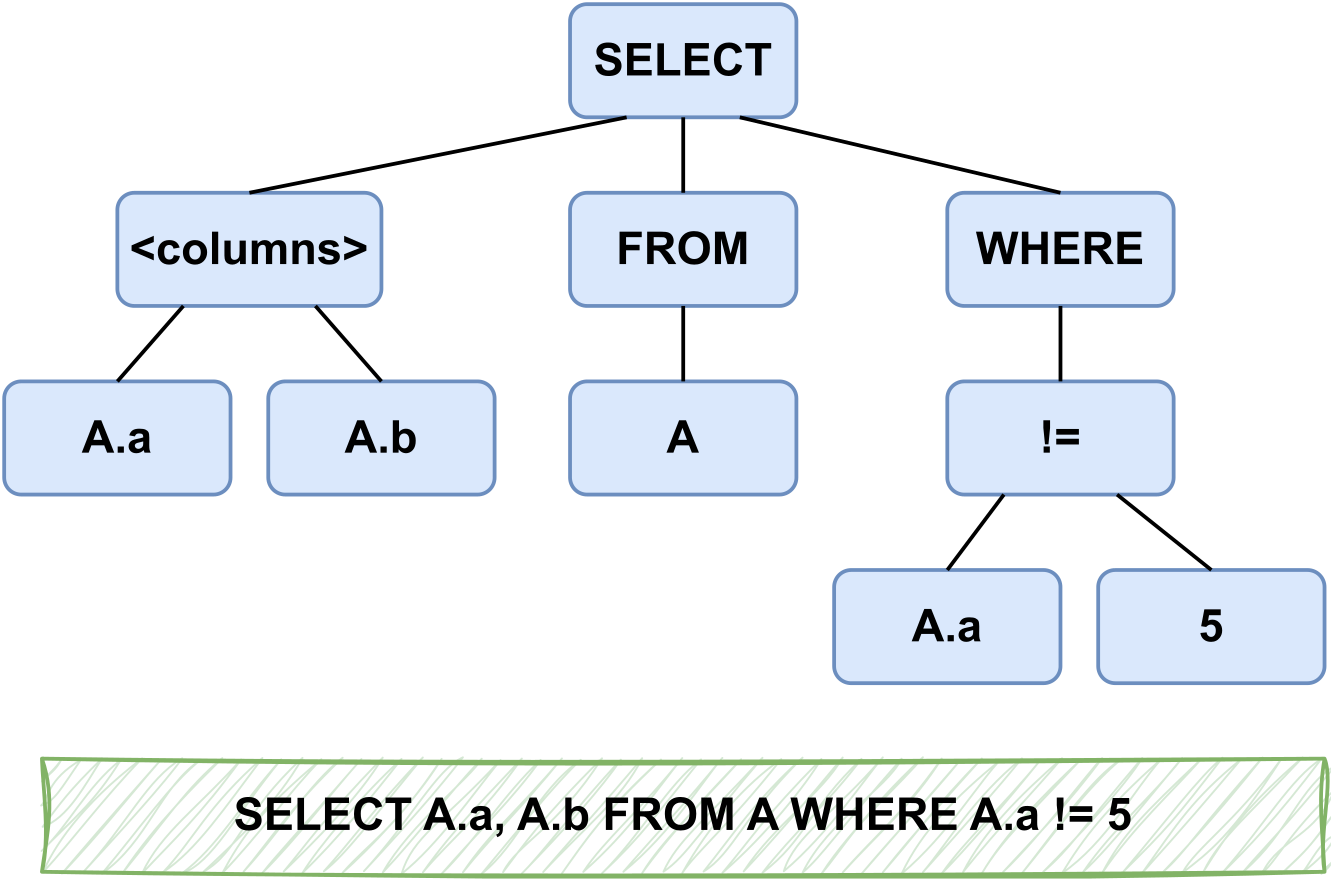
\includegraphics[width=0.55\linewidth]{images/ast_example.png}
  \caption{Drzewo \code{AST} dla przykładowego zapytania SQL}
  \label{fig:sql-ast-example}
\end{figure}

\subsection{Biblioteka Streamlit}
Biblioteka \code{Streamlit}\footnote{\url{https://streamlit.io}} stanowi narzędzie do szybkiego tworzenia interaktywnych aplikacji internetowych opartych na danych. Została zaprojektowana z myślą o prostocie użycia, umożliwiając nawet początkującym programistom szybkie tworzenie interfejsów graficznych, bez konieczności dużej wiedzy na temat frontendu. 

\code{Streamlit} oferuje intuicyjną składnię, która umożliwia tworzenie aplikacji poprzez strumieniowe przetwarzanie danych. Zapewnia integrację z wieloma bibliotekami do analizy danych i uczenia maszynowego. Jedną z kluczowych cech \code{Streamlit} jest automatyczne odświeżanie interfejsu użytkownika w odpowiedzi na zmiany w kodzie, co pozwala na szybką iterację i testowanie aplikacji. Dodatkowo biblioteka oferuje szeroki zakres interaktywnych elementów interfejsu, takich jak suwaki, pola wyboru, czy wykresy, które mogą być łatwo integrowane z analizowanymi danymi. W kontekście niniejszej pracy magisterskiej biblioteka \code{Streamlit} została wykorzystana w celu stworzenia aplikacji pozwalającej na praktyczne wykorzystanie opracowanych rozwiązań.

\section{Visual Studio Code}
Visual Studio Code\footnote{\url{https://code.visualstudio.com}} to wszechstronny edytor stworzony przez Microsoft. Zgodnie z wcześniej wspomnianą ankietą \bibtitle{2023 Developer Survey} \mycite{stackoverflow-survey} jest on najczęściej wybieranym przez deweloperów środowiskiem programistycznym. Tym, co je wyróżnia, jest prostota przy jednoczesnej potędze płynącej z niespotykanej elastyczności. Dostępna jest bowiem ogromna liczba łatwych w instalacji rozszerzeń. Pozwalają one dostosować to środowisko niemal do każdego scenariusza wykorzystania.

Podczas realizacji pracy szczególnie użyteczne okazały się rozszerzenia dla języka Python dodające kolorowanie składni, dokończanie kodu, debugowanie, czy też wsparcie dla interaktywnych notesów \code{Jupyter}. Poza tym intensywnie wykorzystywane było rozszerzenie do pracy z narzędziem \code{Docker}. Jeśli chodzi o podstawowe funkcje środowiska, to bardzo użyteczna okazała się integracja z systemem kontroli wersji oraz zaawansowane wyszukiwanie i zastępowanie.

\section{Docker}
\code{Docker}\footnote{\url{https://www.docker.com}} to bardzo potężne i powszechnie wykorzystywane narzędzie, na którym opiera się znaczna część funkcjonującego oprogramowania. Umożliwia on tworzenie, zarządzanie i uruchamianie aplikacji w niemal całkowicie izolowanych środowiskach zwanych kontenerach. Pozwalają one deweloperom na zapakowanie aplikacji z zależnościami i środowiskiem uruchomieniowym, co zapewnia spójność działania na różnych platformach.

Podczas realizacji niniejszego projektu \code{Docker} okazał się szczególnie użyteczny w kontekście uruchamiania istniejących modeli uczenia maszynowego. Część z nich była od razu gotowa do działania w kontenerze, a inne zostały do tego przystosowane. Okres czasu, w którym analizowane w dalszej części pracy rozwiązania powstawały jest bowiem bardzo rozległy, więc zależności z których korzystają znacznie się różnią i trudno jest je ze sobą pogodzić. W przypadku prostych różnic w pakietach języka Python możliwe jest skorzystanie ze znacznie prostszego narzędzia \code{Conda}, lecz poziom izolacji tworzonych za jego pomocą środowisk jest znacznie ograniczony i jak się okazało często niewystarczający.


\chapter{Przegląd istniejących zbiorów}
Zbiory danych w kontekście uczenia maszynowego stanowią fundamentalny element, wymagany do podejmowania wszelakich problemów. Mają bardzo duży wpływ na skuteczność każdego modelu i z tego powodu przed przystąpieniem do tworzenia polskich odpowiedników zostało poświęcone wiele wysiłku na przeanalizowanie zbiorów istniejących.

Na początku bieżącego rozdziału dokładnie przedstawiony zostanie zbiór \code{Spider}, ze szczególnym zwróceniem uwagi na jego format, którego polskie zbiory będą musiały przestrzegać. W kolejnej części nastąpi przegląd zbiorów do niego pokrewnych, czyli takich, które powstały na fundamencie baz danych \code{Spider} i również odegrały w niniejszej pracy istotną rolę. Na koniec nastąpi dogłębna analiza istniejących tłumaczeń zbioru \code{Spider}, aby dokonać świadomych decyzji podczas tworzenia tłumaczenia polskiego.

\section{Angielski Spider}
\code{Spider} to przede wszystkim zbiór danych przeznaczony do zadania \code{Text-to-SQL}, ale również wyzwanie z publicznie dostępnym rankingiem\furl{https://yale-lily.github.io/spider}, które pozwala konkurować badaczom w tworzeniu coraz lepszych modeli oraz śledzić czynione postępy na przestrzeni czasu.

Na zbiór składa się \numprint{10181} próbek, które są podzielone na trzy części: treningową, walidacyjną (zwaną również deweloperską) oraz testową. Ta ostatnia nie jest jednak powszechnie dostępna i sprawność swojego modelu można uzyskać na niej jedynie poprzez wysłanie go do wyzwania. Daje to pewność, że przypuszczalnie dobre wyniki wysyłanych modeli nie są skutkiem przypadkowego, ani celowego włączenia próbek testowych do zbioru treningowego, czyli zjawiska tak zwanego wycieku danych. Brak swobodnego dostępu do części testowej sprawia, że w praktyce część walidacyjna często przejmuję jej rolę.

Próbki ze zbioru \code{Spider} opierają się na 200 bazach danych, które są bardzo różnorodne, ponieważ obejmują 138 domen, takich jak uczelnie, programy telewizyjne, czy rząd. W niektórych przypadkach ta sama tematyka poruszana jest przez kilka baz danych, co tłumaczy fakt, że jest ich więcej niż samych domen. Bardzo ważne jest to, że bazy są rozdzielone na poszczególne części zbioru. Między innymi żadna baza wykorzystywana w części treningowej nie jest używana w części walidacyjnej ani testowej. Wymusza to na uczonych za pomocą tego zbioru modelach posiadanie umiejętności uogólniania na nowe domeny.

\subsection{Format zbioru}

Wiele istniejących modeli wykorzystuję zbiór \code{Spider} ze względu na jego unikatowość i co za tym idzie, reprezentowany przez niego format stał się w pewien sposób standardem. Nie jest to prosty format tabelaryczny, jak to wygląda w postaci wielu innych zbiorów, lecz składają się na niego cztery jakościowo różne komponenty. Są to przykłady, poprawne zapytania SQL (ang. gold queries), schemat baz danych oraz same bazy. Nieco uproszczona struktura plików zbioru została przedstawiona na rysunku \ref{fig:spider-structure} 

\begin{figure}[ht]
  \centering
    \begin{forest}
      for tree={
        inner sep=0pt,l=10pt,l sep=10pt,
        font=\ttfamily,
        grow'=0,
        child anchor=west,
        parent anchor=south,
        anchor=west,
        calign=first,
        edge path={
          \noexpand\path [draw, \forestoption{edge}]
          (!u.south west) +(7.5pt,0) |- node[fill,inner sep=1.25pt] {} (.child anchor)\forestoption{edge label};
        },
        before typesetting nodes={
          if n=1
            {insert before={[,phantom]}}
            {}
        },
        fit=band,
        before computing xy={l=15pt},
      }
    [Spider
      [database
        [db1]
        [db2]
        [...]
      ]
      [dev.json]
      [train\_spider.json]
      [train\_others.json]
      [dev\_gold.sql]
      [train\_gold.sql]
      [tables.json]
    ]
    \end{forest}
\caption{Struktura plików zbioru \code{Spider}}
  \label{fig:spider-structure}
\end{figure}

\subsubsection{Próbki (\code{dev.json}, \code{train\_spider.json}, \code{train\_others.json})} 
Próbki przechowywane są w formacie JSON i podzielone zostały na trzy pliki. W \code{dev.json} znajdują się te odpowiadające zbiorowi walidacyjnemu, natomiast w plikach \code{train\_spider.json} oraz \code{train\_others.json} umieszczono próbki treningowe. Są one rozdzielone dodatkowo na dwa pliki, ponieważ w pierwszym twórcy zbioru umieścili swoje autorskie przykłady, natomiast w drugim te wyselekcjonowane z już istniejących zbiorów. Przykładowa próbka została przedstawiona na listingu \ref{lst:spider-sample}.

\begin{minipage}{\linewidth}
\lstinputlisting[
style=json,
caption=Przykładowa próbka ze zbioru \code{Spider},
label={lst:spider-sample},
]{listings/spider_sample.json}
\end{minipage}

Znaczenie poszczególnych atrybutów próbki jest następujące:\nobreakpar
\begin{itemize}
    \item \textbf{\code{db\_id}} -- identyfikator bazy danych,
    \item \textbf{\code{question}} -- pytanie w języku naturalnym,
    \item \textbf{\code{question\_toks}} -- pytanie podzielone na tokeny,
    \item \textbf{\code{query}} -- zapytanie SQL,
    \item \textbf{\code{query\_toks}} -- zapytanie SQL podzielone na tokeny,
    \item \textbf{\code{query\_toks\_no\_value}} -- zapytanie SQL podzielone na tokeny, ale z zamaskowanymi wszystkimi wartościami, a dokładnie zastąpionymi tekstem \code{value},
    \item \textbf{\code{sql}} -- skomplikowany obiekt JSON będący sparsowanym zapytaniem SQL, pozwalający na szybkie liczenie metryk i wydobywanie różnych fragmentów zapytania.
\end{itemize}

\subsubsection{Poprawne zapytania SQL (\code{dev\_gold.sql}, \code{train\_gold.sql})}
Poprawne zapytania SQL, zgodnie z powyższym opisem, stanowią jeden z atrybutów próbek, lecz poza tym są również wyciągnięte do dwóch osobnych plików \code{dev\_gold.sql} oraz \code{train\_gold.sql}, które odpowiadają części walidacyjnej oraz treningowej. W każdej linii tych plików, jak przedstawiono na listingu \ref{lst:spider-gold}, umieszczone jest poprawne zapytanie SQL oraz identyfikator bazy danych oddzielony od zapytania znakiem tabulacji.

\begin{minipage}{\linewidth}
\lstinputlisting[
style=sql,
caption=Fragment pliku \code{dev\_gold.json} zawierającego poprawne zapytania SQL,
label={lst:spider-gold}
]{listings/spider_gold.txt}
\end{minipage}

\subsubsection{Schemat (\code{tables.json})}
Plik \code{tables.json}, którego fragment został przedstawiony na listingu \ref{lst:spider-tables}, opisuję strukturę każdej zawartej w zbiorze \code{Spider} bazy danych. Obejmuję to wskazanie nazw wszystkich tabel i kolumn, typów kolumn, kluczy podstawowych oraz relacji tworzonych przez klucze obce. 

\begin{minipage}{\linewidth}
\lstinputlisting[
style=json,
caption=Fragment pliku \code{tables.json} opisujący schemat pojedynczej bazy danych,
label={lst:spider-tables},
]{listings/spider_tables.json}
\end{minipage}

Znaczenie poszczególnych atrybutów obiektu opisującego schemat bazy danych jest następujące:\nobreakpar
\begin{itemize}
    \item \textbf{\code{db\_id}} -- identyfikator bazy danych,
    \item \textbf{\code{table\_names\_original}} -- nazwy tabel występujących w bazie,
    \item \textbf{\code{table\_names}} -- naturalne odpowiedniki nazw tabel występujących w bazie,
    \item \textbf{\code{column\_names\_original}} -- sekwencja dwuelementowych list zawierających kolejno numer porządkowy tabeli oraz nazwę zawartej w niej kolumny,
    \item \textbf{\code{column\_names}} -- tak jak wyżej, lecz z naturalnymi odpowiednikami nazw kolumn,
    \item \textbf{\code{column\_types}} -- typy danych posiadane przez wyżej wymieniane kolumny,
    \item \textbf{\code{primary\_keys}} -- numery porządkowe kolumn będących kluczami podstawowymi,
    \item \textbf{\code{foreign\_keys}} -- sekwencja dwuelementowych list zawierających kolejno numer porządkowy kolumny będącej kluczem obcym oraz numer porządkowy kolumny będącej powiązanym kluczem podstawowym.
\end{itemize}

Warto zwrócić uwagę na fakt, że w pliku schematu, oprócz oryginalnie występujących w bazie nazw tabel i kolumn, znajdują się również ich odpowiedniki w języku naturalnym. Oznacza to, że nazwy składające się z kilku słów i zapisywane oryginalnie za pomocą różnych konwencji, takich jak Camel Case (np. \code{playerName}), Snake Case (np. \code{player\_name}), czy Pascal Case (np. \code{PlayerName}) są zamieniane na naturalną postać, czyli słowa odseparowane spacjami. Poza tym część oryginalnie skrótowych nazw jest rozwijana do bardziej zrozumiałej postaci. Stanowi to dodatkową informację, która nie jest dostępna w samych bazach danych.

\subsubsection{Bazy danych (\code{database/*})}
Ostatnim komponentem zbioru \code{Spider} jest katalog \code{database} zwierający szereg podkatalogów o nazwach odpowiadających identyfikatorom baz danych. Wewnątrz każdego z tych podkatalogów umieszczona jest baza danych \code{SQLite} oraz opcjonalnie dodatkowe pliki, takie jak skrypt SQL pozwalający zbudować daną bazę od zera. Większość baz, z nielicznymi wyjątkami, jest wypełniona danymi. Jest to istotne, ponieważ duża część nowoczesnych algorytmów opiera się na tych danych, by generowane zapytania SQL były dokładniejsze.

\section{Angielskie zbiory pokrewne} \label{text:related-datasets}
Jedną z ważniejszych zasług zbioru \code{Spider} jest zgromadzenie pokaźnej liczby baz danych pochodzących z bardzo różnych domen. Było to trudne, ponieważ stanowią informacje poufne dla wykorzystujących je firm i niewielka ich liczba jest dostępna w sieci. Nic więc dziwnego, że na fundamencie baz danych \code{Spider} powstało kilka kolejnych zbiorów. Doskonałym tego przykładem są zbiory \code{CoSQL} \mycite{cosql} oraz \code{SParC} \mycite{sparc}, gdzie zachowano te same bazy, lecz stworzone zostały całkowicie nowe przykłady. Pojawiło się również odmienne podejście polegające na skonstruowaniu zbiorów pochodnych poprzez dokonanie w próbkach ze zbioru \code{Spider} pewnych ukierunkowanych modyfikacji, czego przykładem są zbiory \code{Spider-Syn} \mycite{Gan2021spidersyn}, \code{Spider-DK} \mycite{Gan2021spiderdk}, czy \code{Dr.Spider} \mycite{Chang2023}.

Jako że część ze wspomnianych powyżej zbiorów pokrewnych do zbioru \code{Spider} odegrało istotną rolę w dalszej części pracy to zostaną one pobieżnie opisane w poniższych sekcjach.

\subsection{Spider-Syn}
\code{Spider-Syn} \mycite{Gan2021spidersyn} jest zbiorem danych powstałym ze zbioru \code{Spider} poprzez zmodyfikowanie próbek w taki sposób, aby ograniczyć dosłowne wymienianie w pytaniach nazw kolumn, tabel i wartości z baz danych. Odzwierciedla to scenariusz w którym z interfejsu tekstowego do bazy korzysta osoba, która dokładnie jej nie zna, więc często posługuje się mimowolnie synonimami. Przykładowa próbka została przedstawiona na listingu \ref{lst:spider-syn-example}. Stworzenie tego typu zbioru było istotne, ponieważ okazało się, że duża część istniejących algorytmów opiera się na powiązywaniu pytania z elementami baz danych poprzez znajdywanie dosłownych powtórzeń i w przedstawionym scenariuszu ich skuteczność radykalnie spada. Zbiór ten posiada część treningową oraz walidacyjną. Można w klasyczny sposób dokonać nauki modeli na części treningowej i ewaluację na części testowej, lecz również popularnym scenariuszem jest trening na zbiorze \code{Spider} i ewaluacja na obu częściach \code{Spider-Syn}.

\begin{minipage}{\linewidth}
\lstinputlisting[
style=json,
caption=Przykład próbki ze zbioru \code{Spider-Syn},
label={lst:spider-syn-example}
]{listings/spider_syn_example.json}
\end{minipage}

\subsection{Spider-DK}
Zbiór danych \code{Spider-DK} \mycite{Gan2021spiderdk} (skrót od ang. Domain Knowledge) został zbudowany na podstawie części testowej \code{Spider} w celu oceny tworzonych modeli pod kątem znajomości wiedzy domenowej. Składa się na niego skromna ilość próbek w liczbie 535, gdzie prawie połowa została wybrana ze zbioru \code{Spider} i przeniesiona bez zmian, a druga połowa powstała poprzez zmodyfikowanie przykładów tak, aby dodać wiedzę domenową. Przykładowa próbka została przedstawiona na listingu \ref{lst:spider-dk-example}. Posiada ona atrybut \code{type}, który wskazuje jeden z pięciu przewidzianych typów wiedzy domenowej. W celu dokładniejszego zrozumienia można odwołać się do artykułu wprowadzającego zbiór \code{Spider-DK}, lecz są one następujące:
\begin{itemize}
    \item \textbf{Typ 1} - pomijanie wymieniania kolumn,
    \item \textbf{Typ 2} - proste wnioskowanie,
    \item \textbf{Typ 3} - synonimy wartości komórek,
    \item \textbf{Typ 4} - generowanie warunków na podstawie słów spoza wartości komórek,
    \item \textbf{Typ 5} - wiedza, która łatwo kłóci się z innymi dziedzinami.
\end{itemize}

\begin{minipage}{\linewidth}
\lstinputlisting[
style=json,
caption={Przykład próbki ze zbioru \code{Spider-DK}},
label={lst:spider-dk-example}
]{listings/spider_dk_example.json}
\end{minipage}

\subsection{SParC}
\code{SParC} \mycite{sparc} jest zbiorem danych zawierającym sekwencje przeplatających się ze sobą pytań w języku naturalnym oraz instrukcji SQL otrzymanych w odpowiedzi. Obejmuje \numprint{4298} sekwencji wiadomości, na które składa się łącznie ponad 12 tysięcy pojedynczych pytań. Są one ze sobą powiązane w obrębie konwersacji i wymagają wykorzystania informacji z poprzednich wiadomości, aby poprawnie sformułować żądane zapytanie SQL. Zbiór ten służy więc do nauki modeli rozwiązujących konwersacyjny wariant problemu \code{Text-to-SQL}. Przykładową konwersację z niego pochodzącą przedstawiono na rysunku \ref{fig:sparc-example}. Widać na niej wyraźnie, że kolejne wiadomości bazują na kontekście wprowadzonym przez wiadomości wcześniejsze.

\begin{figure}[ht!]
  \centering
  \includegraphics[width=0.6\linewidth]{images/sparc_example.png}
  \caption[Przykładowa konwersacja ze zbioru \code{SParC}]{Przykładowa konwersacja ze zbioru \code{SParC}}
  \source{\code{SParC} \mycite{sparc}}
  \label{fig:sparc-example}
\end{figure}

\subsection{CoSQL}
\code{CoSQL} \mycite{cosql} jest zbiorem w znacznym stopniu podobnym do \code{SParC}, ponieważ zawiera dane o charakterze konwersacyjnym. Został do niego dodany jednak kolejny poziom złożoności, gdyż konwersacje nie stanowią już naprzemiennie powtarzających się pytań i instrukcji SQL, lecz powstały w drodze dalece swobodniejszych symulowanych rozmów pomiędzy zwykłymi użytkownikami a ekspertami SQL. Każdy dialog odtwarza realistyczny scenariusz eksploracji bazy danych, w którym użytkownik zadaje pytania, a ekspert stara się na nie odpowiedzieć, wyjaśniając niejednoznaczne kwestie, czy też informując o pytaniach bez odpowiedzi. Gdy pytania użytkownika dają się sformułować w języku SQL to ekspert tego dokonuje i prezentuje wyniki w sposób pozwalający zachować naturalny przebieg interakcji. Przykładowa rozmowa, która to demonstruje, została przedstawiona na rysunku \ref{fig:cosql-example}. Kompletny zbiór liczy \numprint{30000} dialogów podzielonych na część treningową i testową. Łącznie zawierają \numprint{10000} zapytań.

\begin{figure}[ht!]
  \centering
  \includegraphics[width=1.0\linewidth]{images/cosql_example.png}
  \caption[Przykładowa konwersacja ze zbioru \code{CoSQL}]{Przykładowa konwersacja ze zbioru \code{CoSQL}}
  \source{\code{CoSQL} \mycite{cosql}}
  \label{fig:cosql-example}
\end{figure}

\section{Tłumaczenia zbioru Spider}
Tak jak zostało zaznaczone we wprowadzeniu, na chwilę obecną wydaje się istnieć pięć publicznie dostępnych zbiorów będących tłumaczeniami \code{Spider}. Cztery spośród nich dokonuje przekładu na konkretny język, a jeden zawiera tłumaczenia na kilka języków. Wspomniane zbiory jednojęzyczne to chiński \code{CSpider}, wietnamski \code{ViText2SQL}, rosyjski \code{PAUQ} oraz nie posiadający nazwy zbiór portugalski. \code{MultiSpider} to natomiast świeży zbiór, bo upowszechniony przez Microsoft w czasie pisanie niniejszej pracy, który zawiera niezależnie opracowane tłumaczenie chińskie, wietnamskie, niemieckie, francuskie, hiszpańskie oraz japońskie. 

Poza publicznie dostępnymi zbiorami danych natrafiono również na wielojęzyczny zbiór \code{XSpider} \mycite{shi-etal-2022-xricl}, który zgodnie z artykułem zawiera między innymi przekłady na język hindi oraz farsi. Jego autorzy twierdzą w artykule, że wszystkie dane umieszczone zostały we wskazanym repozytorium, lecz jest ono całkowicie puste. Zmiana tego stanu jest wątpliwa biorąc pod uwagę fakt, że artykuł ukazał się już ponad dwa lata temu.

Autorzy wymienionych zbiorów, pomimo wspólnego celu, podeszli do zadania na różne sposoby. Celem poniższych sekcji jest przedyskutowanie kluczowych różnic pomiędzy nimi. Jedną z najistotniejszych jest zastosowany rodzaj tłumaczenia. Rozbieżności zaobserwowano również w kwestii tłumaczenia schematu, zawartości baz danych oraz wartości w zapytaniach. Różnice te zostały zestawione w tabeli \ref{tab:spider-trans-diffs} i zostaną dokładnie omówione.


\begin{table}[ht]
    \centering
    \begin{tabular}{|l|c|c|c|c|}
        \hline
        \thead{Zbiór} & 
        \thead{Rodzaj\\tłumaczenia} &
        \thead{Tłumaczenie\\schematu} &
        \thead{Tłumaczenie\\zawartości\\baz danych} &
        \thead{Tłumaczenie\\wartości w\\zapytaniach} \\
        \hline
        \makecell{Chiński\\{\code{CSpider}}} & Manualne & Nie & Nie & Tak \\
        \hline
        \makecell{Wietnamski\\{\code{ViText2SQL}}} & Manualne & Tak & Nie & Tak \\
        \hline
        \makecell{Portugalski\\{\code{Brak Nazwy}}} & Maszynowe & Tak & Nie & Nie \\
        \hline
        \makecell{Rosyjski\\{\code{PAUQ}}} & Manualne & Nie & Częściowo & Tak \\
        \hline
        \makecell{Wielojęzyczny\\{\code{MultiSpider}}} & Manualne & Tak & Nie & Obie wersje \\
        \hline
        \makecell{Wielojęzyczny\\{\code{XSpider}}} & ------ & Nie & ------ & ------ \\
        \hline
    \end{tabular}
    \lcaption{Zestawienie kluczowych różnic pomiędzy tłumaczeniami zbioru \code{Spider}}{Pozioma kreska oznacza brak informacji na dany temat.}
    \label{tab:spider-trans-diffs}
\end{table}

\subsection{Rodzaj tłumaczenia} \label{text:translation-method}
Tłumaczenie maszynowe i manualne to dwa oczywiste podejścia. Pierwsze sprowadza się do wykorzystania gotowych narzędzi, dostępnych najczęściej za pomocą webowych API, takich jak \code{Google Cloud Translation API} \mycite{google-translation-api}, czy \code{DeepL} \mycite{deepl}. Drugie natomiast oznacza ręczne tłumaczenie każdej próbki przez człowieka. Oczywiście tłumaczenie ręczne może być wspomagane przez metodę maszynową, aby ograniczyć się do poprawiania tłumaczeń, zamiast pisania ich od początku.

Największą zaletą tłumaczenia maszynowego jest szybkie uzyskanie przetłumaczonego zbioru. Wiąże się to najczęściej z naliczeniem pewnych kosztów, o których należy wspomnieć, lecz mimo wszystko koszt ten jest niewspółmierny do ceny wynajęcia profesjonalnego ludzkiego tłumacza. Jest on również niewiele znaczący w stosunku do czasu, który trzeba by poświęcić, by dokonać tłumaczenia samemu.

Tłumaczenie maszynowe ma jednak istotne wady -- pomimo że dostępne narzędzia stają się coraz lepsze, to wciąż nie dorównują człowiekowi. Sprawia to, że uzyskiwane zbiory danych są bezsprzecznie niższej jakości. Narzędzia te dokonując tłumaczenia zbioru \code{Spider} nie biorą pod uwagę wielu istotnych elementów, które ludzki adnotator by uwzględnił. Przykładem jest ignorowanie domeny podczas tłumaczenia pytania naturalnego. Ludzki tłumacz pytanie \textit{list all parties} w domenie politycznej przetłumaczy jako \textit{zwróć wszystkie partie}. Tłumacz maszynowy natomiast może to przetłumaczyć jako \textit{zwróć wszystkie imprezy}.

Dotychczasowe tłumaczenia zbioru \code{Spider}, z powodu ograniczeń metody maszynowej, w większości korzystają z ręcznego tłumaczenia zbioru. Jest to prawdą dla rosyjskiego \code{PAUQ}, wietnamskiego \code{ViText2SQL}, chińskiego \code{CSpider} oraz \code{MultiSpider}. Autorzy części z tych manualnie tłumaczonych zbiorów dla porównania dokonali również tłumaczenia maszynowego. Zestawienie wyników osiąganych przez modele trenowane na zbiorach tłumaczonych maszynowo i manualnie zostało przedstawione w tabeli \ref{tab:manual-vs-machine}. Wszystkie wyniki potwierdzają, że tłumaczenie manualne pozwala uzyskać lepsze rezultaty, aczkolwiek w przypadku względnie nowych modeli \code{RAT-SQL} oraz \code{BRIDGE} procentowy spadek skuteczności na zbiorach maszynowych nie jest tak znaczący, jak dla modeli wcześniejszych.

\begin{table}[ht]
    \centering
    \begin{tabular}{|l|l|R{0.15\textwidth}|R{0.15\textwidth}|R{0.15\textwidth}|}
        \hline
        \thead{Zbiór} & \thead{Model} & \thead{Maszynowe} & \thead{Manualne} &
        \thead{Różnica} \\
        \hline
        \code{CSpider} & C-ML & \s7,9 & 12,1 & \s4,1 \\
        \hline
        \code{CSpider} & W-ML & \s0,6 & 10,0 & \s2,4 \\
        \hline
        \code{ViText2SQL} & EditSQL (Vi-Syllable) & 16,8 & 24,1 & \s7,3 \\
        \hline
        \code{ViText2SQL} & EditSQL (Vi-Word) & 17,4 & 30,2 & 12,8 \\
        \hline
        \code{PAUQ} & RAT-SQL & 46,0 & 51,0 & \s5,0 \\
        \hline
        \code{PAUQ} & BRIDGE & 49,0 & 52,0 & \s3,0 \\
        \hline
    \end{tabular}
    \lcaption{Wyniki modeli trenowanych na zbiorach tłumaczonych manualnie i maszynowo}{W trzech ostatnich kolumnach zamieszczono wyrażoną procentowo metrykę Exact Match without values, która zostanie dokładnie opisana w części \ref{section:metrics}. Wyższe wartości metryki oznaczają lepsze rezultaty.}
    % \caption[Zestawienie wyników dla tłumaczeń maszynowych i manualnych.]{Zestawienie wyników metryki exact match na części testowej dla tłumaczeń maszynowych i manualnych.}
    \label{tab:manual-vs-machine}
\end{table}

\subsection{Tłumaczenie schematu}
Kolejną kwestią dokonującą podziału wśród istniejących tłumaczeń zbioru \code{Spider} jest obrane podejście co do wynikowego języka schematu baz danych, czyli nazw tabel i kolumn -- mogą być one tłumaczone, albo pozostawione bez zmian w języku angielskim. Drugie podejście jest uzasadnione faktem, że w praktyce, niezależnie od kraju, schemat baz danych jest często utrzymywany w języku angielskim. Ma to takie zalety jak ułatwienie pracy wielonarodowemu zespołowi, czy też uniknięcie problemu ze znakami diakrytycznymi, których wykorzystywanie może być niemożliwe lub utrudnione.

Fakt, że w praktyce nazwy tabel i kolumn zapisywane są w języku angielskim w swoich artykułach wyraźnie podkreślili autorzy tłumaczenia chińskiego, rosyjskiego oraz w pewnym stopniu zbioru \code{XSpider} i z uwagi na to postanowili schematu nie tłumaczyć. Twórcy zbioru wietnamskiego, portugalskiego oraz \code{MultiSpider} postanowili jednak tłumaczenia dokonać, nie przedstawiając dla takiego podejścia specjalnego uzasadnienia.

Należy zauważyć, że reprezentowanie pytań i schematu baz danych w dwóch różnych językach znacząco komplikuje rozwiązywany problem. W wariancie ze wszystkimi komponentami w tym samym języku dość łatwo jest znaleźć powiązania pomiędzy nimi, ponieważ wystarczy przeanalizować ich podobieństwo jako łańcuchów znaków. W przeciwnym przypadku to jednak nie wystarczy -- wykorzystywany model musi przejawiać dodatkowo pewne cechy tłumacza.

Podsumowując, pozostawienie schematu baz danych w języku angielskim jest uzasadnione z praktycznego punktu widzenia, jednak dodatkowo komplikuje zadanie. Zbiór danych z przetłumaczonym schematem, chociaż w dużym stopniu ignoruje aspekt praktyczny, stanowi lepszy odpowiednik oryginalnego zbioru \code{Spider} i pozwala na wykonywanie względem niego bardziej sprawiedliwych porównań.

\subsection{Tłumaczenie zawartości baz danych}
Kolejną niespójnością jaką można zaobserwować pomiędzy istniejącymi tłumaczeniami zbioru \code{Spider} jest kwestia tłumaczenia zawartości baz danych. Dokonanie takiego tłumaczenia ma istotne zalety przedstawione w kolejnych akapitach, jednak jest to zadanie problematyczne, przez co nie wszyscy autorzy zbiorów się go podjęli.

Większość nowych podejść do problemu generowania SQL analizuje znajdujące się w bazach danych rekordy, aby zwiększyć swoją skuteczność. Przykładowo użytkownik systemu może poprosić o zwrócenie populacji Polski, a dwie możliwe odpowiedzi mogłyby zawierać fragmenty \sql{WHERE country = 'PL'} oraz \sql{WHERE country = 'polska'}. Widać tutaj, że schemat bazy nie mówi wszystkiego i bez dostępu do jej zawartości obie odpowiedzi są równie dobre, choć tylko jedna poprawna. W celu wytrenowania najlepszych modeli przygotowany zbiór powinien zawierać wypełnione bazy danych, a większość istniejących modeli korzystających z zawartości bazy, zakłada, że jest ona w tym samym języku co pytania.

Drugim zastosowaniem wartości w bazach danych jest umożliwienie ewaluacji przygotowanych algorytmów przy pomocy metryki execution accuracy. Została ona opisana dokładnie w dalszej części pracy w sekcji x.xx. Jej skrótowa zasada działania polega na wykonaniu prawidłowych zapytań oraz zapytań wygenerowanych i uznaniu poprawnymi tych, które zwróciły te same wyniki. Przetłumaczenie wartości w zapytaniach SQL bez tłumaczenia zawartości baz danych skutkuję tym, że wykonywane zapytania często nie zwracają żadnych wyników, a co za tym idzie, wiele nieprawidłowo wygenerowanych zapytań jest uznawanych omyłkowo za prawidłowe. Podsumowując, różne języki wartości w zapytaniach SQL i wartości w bazach danych skutkują upośledzeniem metryki execution accuracy i zmniejszeniem jej użyteczności.

Wśród przedstawionych wersji zbioru \code{Spider} modyfikacji zawartości bazy danych podjęli się jedynie autorzy tłumaczenia rosyjskiego. Nie tłumaczyli oni jednak wszystkich wartości, ale tylko te, które wystąpiły w przynajmniej jednym zapytaniu. Powodem dla którego pozostałe zbiory obyły się bez tłumaczenia zapewne jest duża liczba danych zawartych w bazach i relatywnie niewielkie korzyści wynikające z ich tłumaczenia. Autorzy zbioru portugalskiego rozwiązali ten problem w jeszcze inny sposób - postanowili nie tłumaczyć wartości w zapytaniach, dzięki czemu znajdujące się w nich wartości i w bazach danych były w tym samym języku. Takie podejście wydaje się jednak naciągane, bo mało praktyczne - zakłada scenariusz w których w bazach danych o portugalskim schemacie przechowywane są wartości angielskie.


\chapter{Tworzenie polskich zbiorów}
W ostatnim czasie w szczególności nacisk zostaje przenoszony z modeli na odpowiednie przygotowanie i jakość zbiorów danych. Przykładem tego jest wydany w ostatnim czasie artykuł \bibtitle{Textbooks are all you need} \cite{Gunasekar2023}, który demonstruję jak dużą poprawę można uzyskać bez powiększania i komplikowania wykorzystywanego modelu, lecz poprzez stworzenie wysokiej jakości zbioru danych.

Jako, że dla zadania \code{Text-to-SQL} na moment pisania niniejszej pracy nie istnieją żadne zbiory danych w języku polskim, a także ze względu na duże ich znaczenie, wiele uwagi zostało poświęcone tej kwestii. 

Na początku bieżącego rozdziału omówione zostaną przyjęte założenia dotyczące tworzenia polskich zbiorów, a następnie przedyskutowane dokładnie dwa kluczowe dla tego procesu elementy: dynamiczne generowanie oraz sposób dokonywania tłumaczenia. Ostatecznie nastąpi analiza i podsumowanie stworzonych zbiorów.

\section{Przyjęte założenia}
Po przeanalizowaniu różnic pomiędzy istniejącymi tłumaczeniami zbioru \code{Spider} określone zostały założenia przyjęte na potrzebę stworzenia zbiorów polskich.

% To fix:
Podczas tłumaczenia zbiorów przyjęto dwa podstawowe założenia. Pierwszym jest wykorzystanie tłumaczenia maszynowego, zamiast manualnego. Drugi stanowi dynamiczne generowanie finalnych zbiorów zamiast jednorazowego tłumaczenia wszystkich przykładów i udostępnienia jedynie zmodyfikowanej ich wersji. Oba założenia zostaną rozwinięte, uzasadnione i dokładnie przedyskutowane w poniższych dwóch sekcjach.

\subsection{Tłumaczenie maszynowe}
Pomimo wskazanej w sekcji \ref{text:translation-method} dominacji tłumaczenia manualnego nad maszynowym postanowiono wykorzystać to ostatnie. Przyczyn tej decyzji jest kilka. Przede wszystkim w realizację tłumaczenia aktywnie zaangażowana jest tylko jedna osoba, w odróżnieniu do wcześniejszych prac, w których w tym procesie uczestniczyło ich kilka, a w przypadku rosyjskiego zbioru nawet profesjonalny tłumacz. Drugą przesłanką jest ograniczony czas, ze względu na pracę magisterką w ramach której niniejszy temat jest realizowany. Ostatecznie jest to zadanie żmudne, a zbiór maszynowy, pomimo niższej jakości, także pozwoli, a nawet da więcej czasu, na wykonanie eksperymentów.

\subsection{Generowanie zbiorów}
Wszystkie dotychczasowe tłumaczenia zbioru Spider sprowadzają się jedynie do udostępnienia zmodyfikowanej wersji zbioru, bez żadnych dodatkowych skryptów. Wydaje się to wystarczające i dla większości zastosowań w rzeczywistości jest. Taki zbiór stanowi bardzo dobry benchmark służący do porównywania różnych algorytmów, ponieważ nie ma żadnych niedomówień w kwestii jego zawartości.

W niniejszej pracy zaproponowano dość innowacyjne, bo niespotykane we wcześniejszych zbiorach podejście, polegające na skryptowym generowaniu zbiorów w żądanej konfiguracji. Na początku zostaną one rozbite na elementarne składniki, czyli pytania, zapytania SQL oraz schematy baz danych. Następnie będzie można przeprowadzić syntezę tych komponentów w kompletny zbiór wybierając przy tym język pytań, język zapytań oraz jedną z możliwych wersji schematu baz danych.

Zdecydowano się na opracowanie takiej metody, gdyż zauważono, że ma ona szereg zalet. Po pierwsze nie trzeba decydować się czy tłumaczyć nazwy tabel i kolumn, czy nie, jak to robili dotychczasowi autorzy tłumaczeń, a nie byli co do tego zgodni. Opisanym sposobem można stworzyć kilka mapowań starych nazw na nowe i do syntezy wykorzystać to, które będzie w danym przypadku najlepsze. Jest to poza zakresem pracy, ale znacząco to ułatwia również tłumaczenia zbioru na inne języki, bo wszystkie komponenty zostały już rozplątane. Generalnie taka strategia jest bardzo elastyczna i otwiera drogę na nowe eksperymenty.

\subsection{Tłumaczenie zbiorów pokrewnych}
Oprócz przetłumaczenia zbioru \code{Spider} postanowiono dokonać tego również dla czterech zbiorów pokrewnych przedstawionych wcześniej w sekcji \ref{text:related-datasets}. Prostym powodem tego jest chęć zdobycia większej liczby próbek w nadziei, że pozwoli to finalnie na wytrenowali lepszej jakości modeli. Poza tym przetłumaczenie \code{Spider-Syn} oraz \code{Spider-DK} pozwoli na testowanie tworzonych algorytmów pod kontem odporności na synonimy, czy znajomości wiedzy domenowej. 

Przetłumaczenie dodatkowych zbiorów jest ułatwione, ponieważ dzięki współdzielonym bazą danych translacji nazw tabel i kolumn wystarczy dokonać jednorazowo. Zastosowane podejście polegające na skryptowym generowaniu ostatecznych zbiorów jeszcze bardziej uprasza ten proces, więc postanowiono to wykorzystać. Nie znaleziono informacji na temat wcześniejszych prób tłumaczenia tych zbiorów, więc niniejsza praca być może jest pierwsza.

\subsection{Oryginalna zawartość baz danych}
Zawartość baz danych postanowiono pozostawić bez zmian - ewentualnemu tłumaczeniu podlegać będzie jedynie ich schemat. Powodem do tego jest duża ilość znajdujących się tam informacji, których tłumaczenie maszynowe skutkowałoby naliczeniem istotnych opłat. Jest to jednocześnie działanie pokrywające się z większością istniejących podejść do tłumaczenia zbioru \code{Spider}. Pomimo pozostawienia oryginalnej zawartości baz danych, modele trenowane na nich wciąż są w stanie osiągać wysokie wyniki, co potwierdza słuszność tego podejścia.

\section{Przygotowanie zbiorów angielskich}
Poza angielskim zbiorem \code{Spider}, którego przetłumaczenie bez wątpienia było najistotniejsze, przetłumaczono również zbiory \code{Spider-Syn}, \code{Spider-DK}, \code{SParC} oraz \code{CoSQL}. Ich struktura oraz przeznaczenie znacząco odbiega od zbioru \code{Spider} i aby je wykorzystać podjęte zostały dodatkowe kroki, które zostały w niniejszej części podsumowane. Niektóre z nich były konieczne, jak zamiana zbiorów z kontekstowych na bezkontekstowe, a inne opcjonalne, jak deduplikacja poprawiająca efektywność nauki modeli. Kroki te sprawiają jednak, że tłumaczenia owych dodatkowych zbiorów nie stanowią idealnych odpowiedników oryginałów. W różnym stopniu, ale należy traktować je jako nowe zbiory i unikać zestawiania osiąganych na nich rezultatów z angielskimi oryginałami.

\subsection{Konwersja zbiorów kontekstowych na bezkontekstowe}
W ramach realizowanego tematu rozważany jest problem tłumaczenia bezkontekstowego, co jest pozornie sprzeczne z wykorzystaniem zbiorów \code{SParC} oraz \code{CoSQL}. Nie zawierają one bowiem prostego szeregu pytań i odpowiadających im zapytań SQL, lecz dodatkowo porządkują je w konwersacje, gdzie kolejne wiadomości bazują na znajomości poprzednich. Zauważono, jednak że zbiory kontekstowe mogą zostać przekonwertowane na bezkontekstowe poprzez wybranie z każdej konwersacji jedynie pierwszego pytania i odpowiedzi. Nie istnieje wówczas żadna historia wcześniejszych wiadomości, więc takie przykłady nie posiadają żadnego dodatkowego kontekstu. Powstałe w ten sposób zbiory znacznie różnią się od oryginalnie kontekstowych zbiorów \code{SParC} oraz \code{CoSQL}, więc całkowicie nieuzasadnionym by było zestawianie ze sobą osiąganych na nich wyników.

\subsection{Modyfikacja pytań}
Część pytań wewnątrz zamienionych już na bezkontekstowe zbiorów \code{SParC} oraz \code{CoSQL} wyraźnie odróżniała się od reszty. Zawierały one bowiem wyrażenia charakterystyczne dla konwersacji, takie jak \enquote{Hi}, \enquote{Hello}, \enquote{How are you}. Są one dla rozważanego problemu niepożądane, bo nie stanowią typowych pytań, które użytkownik wprowadziłby do systemu wiedząc, że zwraca on jedynie zapytania SQL. Z tego powodu postanowiono znaleźć takie wystąpienia za pomocą wyrażeń regularnych oraz funkcji wyszukiwania dostępnej wewnątrz wykorzystywanego edytora i usunąć niepotrzebne fragmenty.

\subsection{Deduplikacja w obrębie zbiorów}
Jako zduplikowane zostały uznane przykłady, które posiadają identyczną bazę danych oraz takie same znormalizowane angielskie pytania (przekonwertowane na małe litery i bez niepotrzebnych białych znaków). Deduplikacji w obrębie zbiorów dokonano poprzez zwyczajne usunięcie występujących kilkukrotnie próbek. Okazało się, że znaleziono takie w każdym ze zbiorów, poza \code{Spider-DK}. 25 przypadków zostało zlokalizowanych nawet w samym zbiorze \code{Spider}, lecz w nim modyfikacji nie wprowadzano, bo ze względu na jego wysoką renomę chciano, by próbki w polskim wariancie dokładnie mu odpowiadały. Najwięcej duplikatów zostało znalezionych w zbiorze \code{SParC}. Widocznie w tym oryginalnie kontekstowym zbiorze wiele konwersacji rozpoczynało się od tych samych wiadomości i różnice następowały dopiero później.

\subsection{Deduplikacja pomiędzy zbiorami}
Istotnym problemem okazały się duplikaty pomiędzy zbiorami. W większości występowały one między \code{Spider}, a całą resztą, ponieważ \code{Spider} powstał jako pierwszy. Widać to doskonale na rysunku \ref{fig:deduplication-before}, gdyż największa liczba duplikatów znajduje się w wierszu oraz kolumnie odpowiadającej właśnie zbiorowi \code{Spider}. Dużą liczbą powtórzeń wyróżnia się w szczególności para zbiorów \code{Spider} oraz \code{Spider-Syn}, ponieważ w tym ostatnim autorzy umieszczali oryginalną próbkę, jeżeli nie udało im się wymyślić rozsądnego synonimu. Ostatecznie całą duplikację ze zbiorem \code{Spider} postanowiono usunąć. Jedynym wyjątkiem są powtórzenia pomiędzy parą \code{Spider-DK} oraz \code{Spider}, które pozostawiono, ponieważ \code{Spider-DK} ma charakter czysto walidacyjny i 206 znalezionych duplikatów to nie przypadkowe próbki, lecz precyzyjnie wyselekcjonowane ze zbioru \code{Spider} przykłady zawierające wiedze domenową. Pozostawioną w zbiorach duplikację po usunięciu części próbek przedstawiono na rysunku \ref{fig:deduplication-after}. 

\begin{figure}[ht!]
\centering
\begin{subfigure}{0.49\textwidth}
    \includegraphics[width=\textwidth]{images/duplicates_before.png}
    \caption{Przed deduplikacją}
    \label{fig:deduplication-before}
\end{subfigure}
\hfill
\begin{subfigure}{0.49\textwidth}
    \includegraphics[width=\textwidth]{images/duplicates_after.png}
    \caption{Po deduplikacji}
    \label{fig:deduplication-after}
\end{subfigure}
\caption[Diagramy ilustrujące liczbę duplikatów pomiędzy zbiorami]{Diagramy ilustrujące liczbę duplikatów pomiędzy zbiorami - na osiach umieszczono nazwy zbiorów wraz z liczbą próbek, a wartości w komórkach macierzy wskazują liczbie duplikatów pomiędzy daną parą zbiorów.}
\label{fig:cross-dataset-duplicates}
\end{figure}

\subsection{Deduplikacja tłumaczeń}
Deduplikacja tłumaczeń to działanie, które dotyczy wyłącznie zbioru \code{Spider-Syn}. Trzeba zauważyć, że opisane powyżej usuwanie duplikatów bazuje na angielskich wersjach pytań, co wydaję się wystarczające, ponieważ jeżeli pytania angielskie się różnią, to ich polskie tłumaczenia również powinny się różnić. W przypadku próbek zawartych w zbiorze \code{Spider-Syn} jest jednak często inaczej. Dla przypomnienia, zawiera on próbki z oryginalnego zbioru \code{Spider}, lecz z wybranymi słowami zamienionymi na synonimy. Okazuje się, że te synonimy oraz bazowe słowa od których pochodzą tłumaczone są niejednokrotnie przez \code{DeepL} na te same polskie wyrażenia, co skutkuje duplikatami w liczbie 1350. Proces ich powstawania został zilustrowany na rysunku \ref{fig:deduplication-after-translation}. Aby pozbyć się tak powstałej duplikacji postanowiono usunąć niepotrzebne próbki ze zbioru \code{Spider-Syn}. Działanie to, w odróżnieniu do wcześniej opisanych, musiało się odbyć już po dokonaniu tłumaczenia na język polski.

\begin{figure}[ht!]
  \centering
  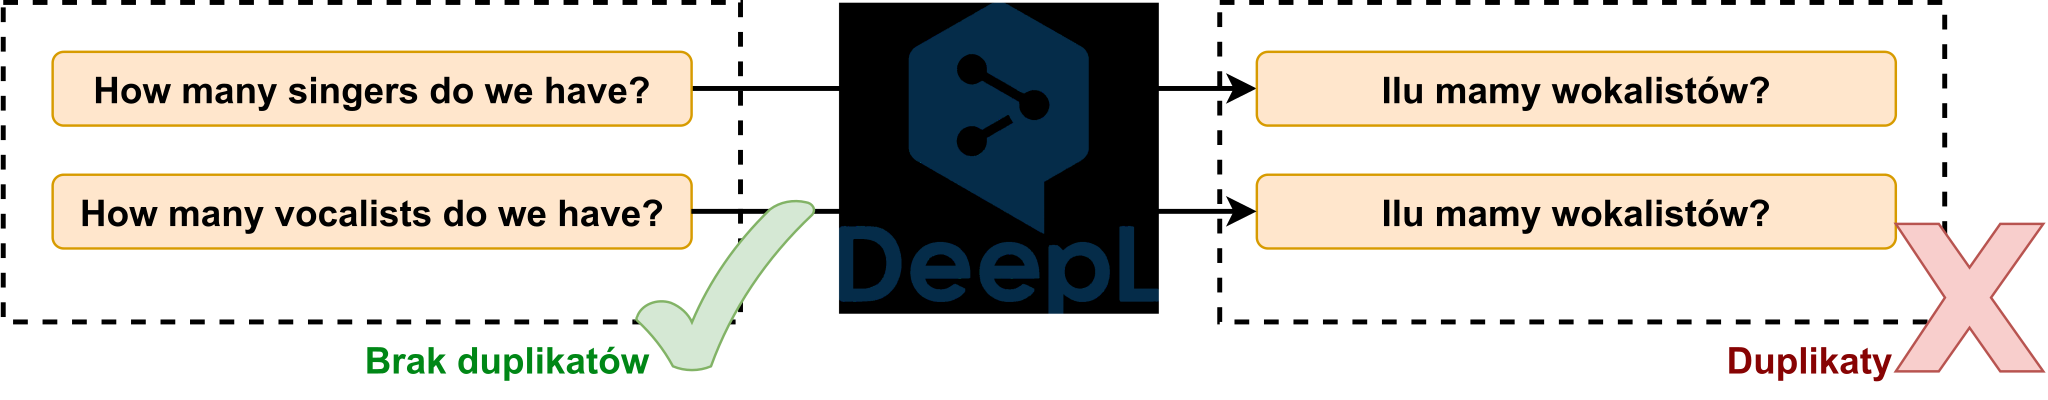
\includegraphics[width=1.0\linewidth]{images/duplication_after_translation.png}
  \caption{Sposób powstawania duplikacji pomiędzy \code{Spider} i \code{Spider-Syn} w wyniku tłumaczenia}
  \label{fig:deduplication-after-translation}
\end{figure}

\section{Generowanie zbiorów}
Generowanie zbiorów w różnych konfiguracjach jest ważnym elementem niniejszej pracy i w znaczny sposób odróżnia ją od wcześniejszych podejść. W związku z tym zostanie ono w tej części dokładnie opisane.

Implementacja tej strategii sprowadza się do stworzenia skryptu pozwalającego na wygenerowanie zbioru o żądanych parametrach. Wśród nich możliwe jest określenie języka pytań, języka wartości w zapytaniach i wariantu tłumaczenia schematu bazy danych.

Na początku przedstawione zostaną nowo wprowadzone formaty plików, które stworzony skrypt wykorzystuję do generowania wariantów zbioru.

\subsection{Dane źródłowe}
Przed przystąpieniem do tworzenia skryptu generującego zbiory w żądanych konfiguracjach konieczne okazało się zastanowienie nad danymi źródłowymi, które będą niezbędne do jego działania. Ostatecznie dane te zostały rozbite na dwa typy plików: próbki, które zawierają alternatywne wersję pytań i zapytań SQL oraz pliki mapowań nazw schematu, które zawierają kompletne mapowania oryginalnych nazw tabel i kolumn na nowe. Formaty tych plików zostały opisane w poniższych sekcjach. Taka dekompozycja umożliwia dodawanie kolejnych zbiorów poprzez tworzenie nowych plików próbek i dodawanie kolejnych sposobów tłumaczenia nazw tabel i kolumn poprzez tworzenie nowych plików mapowań schematu.

\subsubsection{Plik próbek}
Przykładowy element z opracowanego pliku próbek został przedstawiony na listingu \ref{lst:new-sample}. Ma on stanowić bazę na podstawie której będą generowane kompletne zbiory. Każdy zawarty w nim przykład zawiera jedynie niezbędne informacje, czyli nazwę bazy danych oraz alternatywne warianty pytań i zapytań SQL. Przedstawiony przykład zawiera jedynie angielskie i polskie warianty, bo tylko one są istotne dla realizacji niniejszego tematu. Nic nie stoi na przeszkodzie, aby dodać jednak kolejne języki, gdyż zarówno format omawianego pliku, jak i skrypt generujący został na taką okoliczność przygotowany.

\begin{minipage}{\linewidth}
\lstinputlisting[
caption=Pojedynczy przykład z opracowanego pliku próbek \code{tables.json} opisujący schemat pojedynczej bazy danych, label={lst:new-sample}, language=json
]{listings/new_sample.json}
\end{minipage}

Warto zwrócić uwagę, że próbki w finalnym zbiorze muszą posiadać znacznie więcej atrybutów niż te przedstawione powyżej. Powinny zawierać dodatkowo pytania i zapytania SQL podzielone na tokeny oraz sparsowane zapytania. Są to jednak w dużej części informacje redundantne, które można z powodzeniem odtworzyć na podstawie skromnych informacji przedstawionych powyżej i jest to jedna z funkcji które będzie realizował skrypt generujący. Sprawia to, że tworzone rozwiązanie jest zgodne z powszechnie cenioną architekturą \code{Single Source of Truth} (SSOT). Polega ona na unikaniu za wszelką cenę powielania tych samych informacji w kilku miejscach, ponieważ, gdy zostaną zmodyfikowane to pojawia się bardzo duże ryzyko powstania niespójności. Istotność tej metodyki w inżynierii oprogramowania została dobrze przedstawiona w artykule \bibtitle{Single Source of Truth (SSOT) for Service Oriented Architecture (SOA)} \cite{Pang2014}.

\subsubsection{Plik mapowań nazw schematu}
Aby umożliwić dokonywanie różnych tłumaczeń schematu baz danych opracowany został format pliku przedstawiony na listingu \ref{lst:new-trans}. Zawiera on informacje pozwalające dokonać mapowania oryginalnych nazw na dowolne inne. Jest to plik json o kilku stopniach zagnieżdżenia. Na najwyższym poziomie jest słownikiem, który dla każdej nazwy bazy zawiera listę tabel, a każda tabela listę kolumn. Wszystkie obiekty reprezentujący tabele i kolumny posiadają docelowe nazwy na jakie powinny zostać przetłumaczone.

\begin{minipage}{\linewidth}
\lstinputlisting[
caption=Fragment opracowanego pliku mapowań nazw schematu, label={lst:new-trans}, language=json
]{listings/new_trans.json}
\end{minipage}

Należy zwrócić uwagę, że format ten pozwala, aby dana kolumna była tłumaczona na różne sposoby w zależności od tabeli i bazy w której się znajduję. Podobnie ta sama nazwa tabeli może być tłumaczona na różne sposoby w zależności od bazy danych. Jest to celowy zabieg i wymagany w celu umożliwienia wysokiej jakości tłumaczenia. Rozważmy dla przykładu tabelę o nazwie \code{department}. W bazie dotyczącej biznesu prawdopodobnie powinna zostać przetłumaczona jako \code{dział}, natomiast w domenie uniwersyteckiej jako \code{wydział}. Przyjęcie bardziej zaawansowanego podejścia umożliwiło dokonanie tego typu tłumaczenia kontekstowego, przedstawionego w dalszej części pracy.

\subsection{Zmiana nazw tabel i kolumn}
Dokonanie zmian nazw w schemacie, z punktu widzenia oryginalnego zbioru Spider, sprowadza się do zmodyfikowania dwóch elementów: samych baz danych oraz schematu wewnątrz zapytań SQL. W poniższych sekcjach zostanie przedstawiony opracowany algorytm, który tego dokonuje wraz z analizą alternatywnych możliwości. 

\subsubsection{Modyfikacje w bazach danych}
Zmodyfikowanie nazw tabel i kolumn w bazach danych nie stanowi dużego wyzwania, ponieważ wystarczy wykonać na każdej z nich serię instrukcji typu \sql{ALTER TABLE}. Przystępując do tego należy jednak upewnić się, że zastosowanie danego mapowanie nie tworzy konfliktujących ze sobą pod względem nazw elementów, bo wówczas operacja się nie powiedzie. Podczas tłumaczenia zauważono także, że należy pomijać tabele o nazwie \code{sqlite\_sequence}, ponieważ jest to specjalna tabela i jej modyfikacja nie jest możliwa.

\subsubsection{Modyfikacje w zapytaniach}
Dokonanie podmiany nazw tabel i kolumn w zapytaniach SQL stanowi najtrudniejszy etap w całym procesie generowania zbioru. Przyczyną tego jest przyjęte podejście polegające na tym, że dana kolumna może być przetłumaczona na różne sposoby, w zależności od tabeli w której się znajduję. W przypadku modyfikacji baz danych było oczywistym do której tabeli należy każda kolumna, bo wynika to z ich jasno zdefiniowanej struktury. Zapytania SQL są natomiast w gruncie rzeczy zwykłymi tekstami i wydobycie z nich kolumn oraz ustalenie tabel do których należą stanowi duże wyzwanie.

Najłatwiejsze podejście do tego problemu, ale posiadające istotny problem, wykorzystuje parsowanie zapytań do postaci drzewa AST (ang. Abstract Syntax Tree). Jest to sposób reprezentacji wyrażenia w języku formalnym, takim jak SQL, za pomocą drzewa, którego przykład został przedstawiony na rysunku \ref{fig:ast-example}. Można z niego wygodnie wydobywać różne informacje, czy też dokonywać modyfikacji. Warto więc na jego poziomie przeprowadzić tłumaczenia nazw, a następnie odwrócić proces parsowania i uzyskać dla zapytania zmodyfikowaną postać tekstową. W wykorzystanym języku Python istnieje popularna biblioteka \code{sqlglot}, która pozwala na wykonywanie tego typu operacji. 

\begin{figure}[ht!]
  \centering
  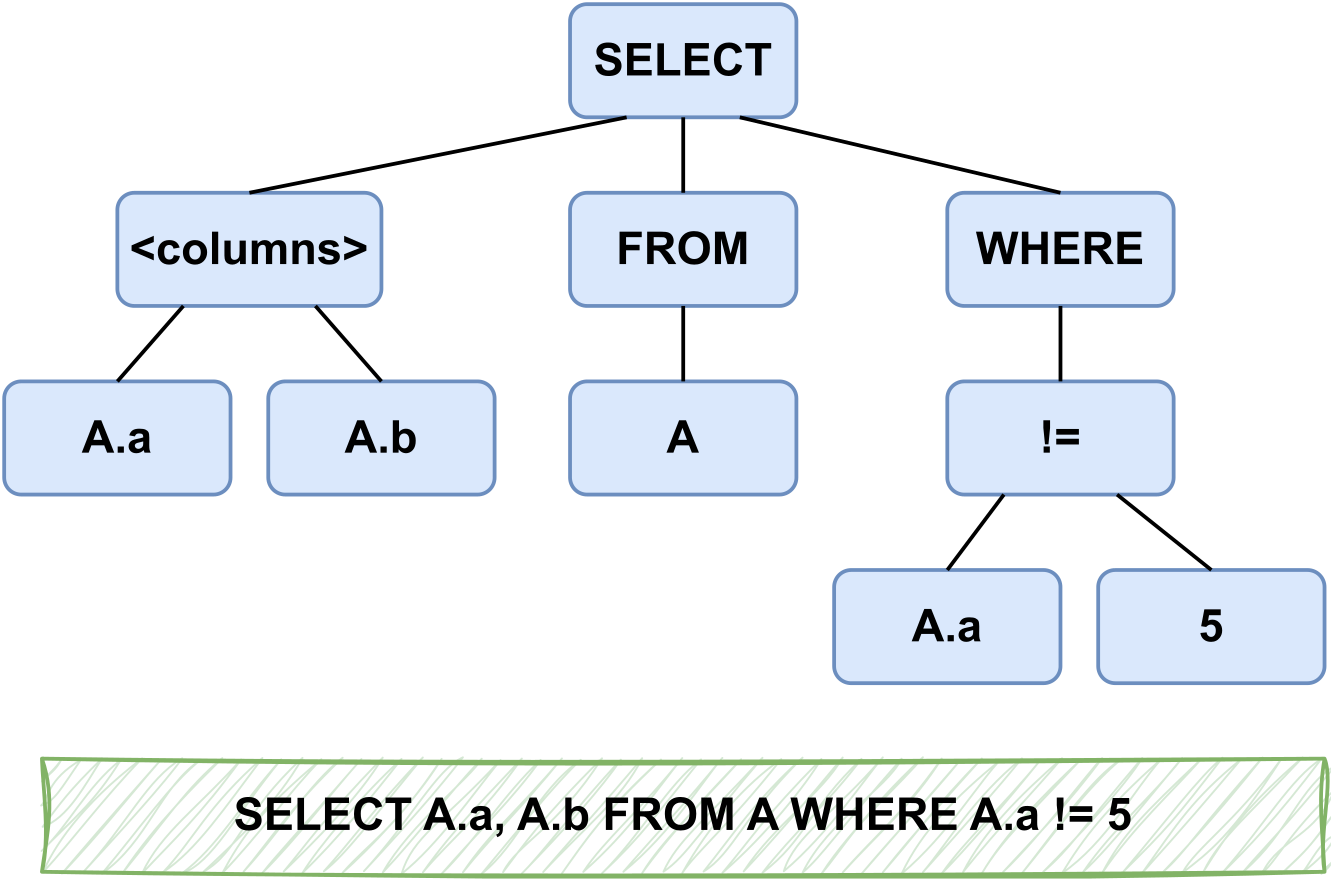
\includegraphics[width=0.6\linewidth]{images/ast_example.png}
  \caption{Drzewo AST dla przykładowego zapytania SQL}
  \label{fig:ast-example}
\end{figure}

Wspomnianym problemem z wykorzystaniem AST jest to, że przetłumaczone z wykorzystaniem biblioteki \code{sqlglot} zapytania, chociaż pod względem semantycznym pozostają bez zmian, to modyfikacji ulega ich formatowanie - następuje zmiana sposobu nawiasowania, czy też stawiania białych znaków. Przekonwertowane w ten sposób zapytania odbiegają więc istotnie od oryginalnych i porównywanie takiego zbioru z oryginalnym \code{Spider} mogło by być kwestionowane. Ponadto wiele algorytmów opiera się na specyficznym dla zbioru \code{Spider} formacie zapytań i jego modyfikacja doprowadziła by do problemów z uruchomieniem wielu modeli. Z przytoczonych powodów porzucono to podejście.

W celu dokonania modyfikacji schematu w zapytaniach, bez niepotrzebnego wpływania na ich strukturę, zdecydowano się ostatecznie zrobić to na niższym poziomie. W tym celu opracowano algorytm, który najpierw dokonuje tokenizacji zapytań, a następnie analizuje wszystkie tokeny po kolei i jeżeli trafi na nazwę kolumny lub tabeli to dokonuję podmiany na nową nazwę. Aby sprawdzić, czy dany token jest nazwą kolumny lub tabeli dokonywano parsowania zapytania do AST, następnie zmieniano dany token na inny i ponownie parsowano zapytanie do AST. Porównując ze sobą te dwa drzewa AST można było ustalić, czy zmodyfikowanym tokenem była nazwa tabeli, nazwa kolumny, czy żadne z powyższych.

W celu przetłumaczenia nazwy kolumny należało dodatkowo ustalić, do jakiej tabeli ona należy. Aby to zrobić konieczne było rozpatrzenie trzech możliwych przypadków:

\begin{enumerate}
    \item Nazwa kolumny poprzedzona nazwą tabeli (\sql{SELECT order.id FROM order})
    \item Nazwa kolumny poprzedzona aliasem (\sql{SELECT T1.id FROM order as T1})
    \item Nazwa kolumny bez tabeli (\sql{SELECT id FROM order})
\end{enumerate}

Pierwszy scenariusz jest najprostszy, ponieważ nazwa tabeli jest jawnie podana i nie ma co do niej wątpliwości. Drugi przypadek jest bardziej skomplikowany ponieważ zamiast istniejącej nazwy tabeli wykorzystany został stworzony alias, więc wcześniej trzeba wydobyć z zapytania wszystkie aliasowania. Trzeci przypadek jest również trudny, ponieważ kolumna należy do jednej z wykorzystanych w zapytaniu tabel, więc trzeba wiedzieć dodatkowo jakie tabele są dostępne. Dla tych dwóch przypadków sytuację dodatkowo komplikuję fakt, że zapytania mogą być swobodnie zagnieżdżanie i łączone szeregowo za pomocą operatorów zbiorowych, co skutkuje tym, że w obrębie pojedynczego zapytania pojawiają się zakresy w których dostępne są różne tabele i różne aliasowania.

Aby poradzić sobie z ustaleniem przynależności kolumn do tabel w skomplikowanych zapytaniach postanowiono więc dokonywać rekurencyjnego rozbijania składających się na nie tokenów, przekazując przy tym kontekst mówiący o obowiązującym aliasowaniu z zapytań nadrzędnych do podrzędnych. Zostało to zilustrowane na rysunkach 
\ref{fig:query-decomposition-serial} oraz \ref{fig:query-decomposition-nested}. Przedstawiają one odpowiednio dekompozycję zapytania zawierającego operator zbiorowy oraz dekompozycję zapytania z zagnieżdżeniem. W tym drugim przypadku miejsce zapytania podrzędnego jest zastępowane poprzez fragment \sql{SELECT 1}, aby zapewnić strukturalną poprawność obu wynikowych zapytań. W wyniku tego procesu otrzymywany jest zbiór elementarnych zapytań wraz z obowiązującymi wewnątrz nich kontekstami, co pozwala na łatwą modyfikację tokenów odpowiadających za nazwy tabel i kolumn. Jako, że pierwotnym źródłem tych tokenów jego wejściowe, skomplikowane zapytanie to również ono jest tłumaczone - niejako jako efekt uboczny, lecz jest to celowym zamierzeniem.

% Podczas tego procesu kontekst z zapytań nadrzędnych, jest przekazywany do zapytań podrzędnych, aby utrzymywać przez cały czas informację o dostępnych w danej części zapytania aliasowaniach.

\begin{figure}[ht!]
  \centering
  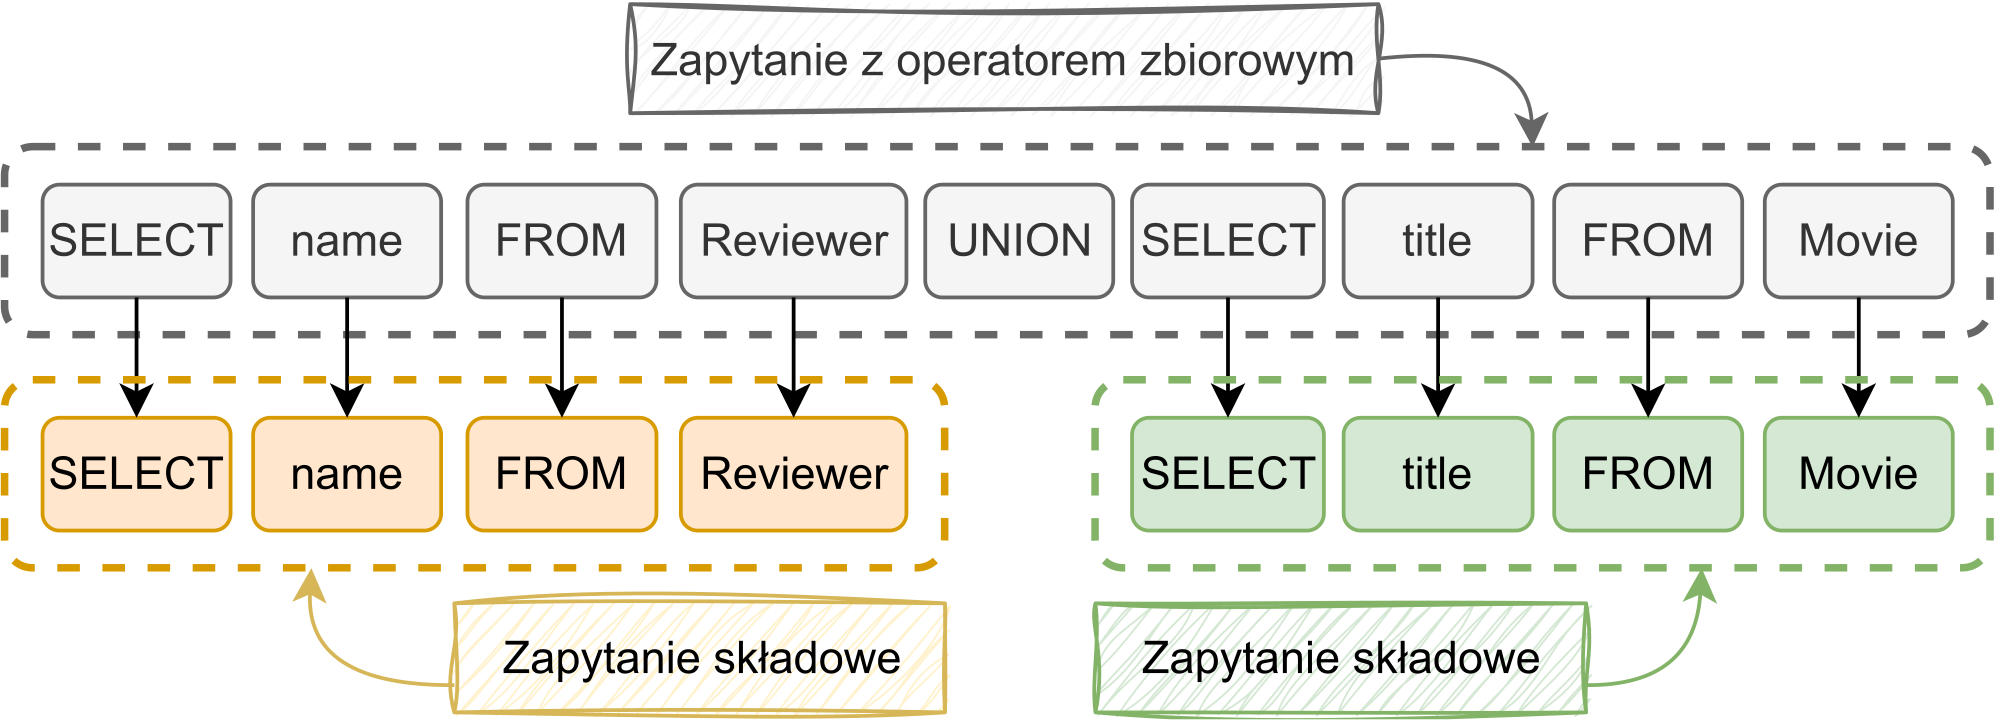
\includegraphics[width=1.0\linewidth]{images/query_decomposition_serial.png}
  \caption{Metoda dekomponowania zapytań z operatorami zbiorowymi}
  \label{fig:query-decomposition-serial}
\end{figure}

\begin{figure}[ht!]
  \centering
  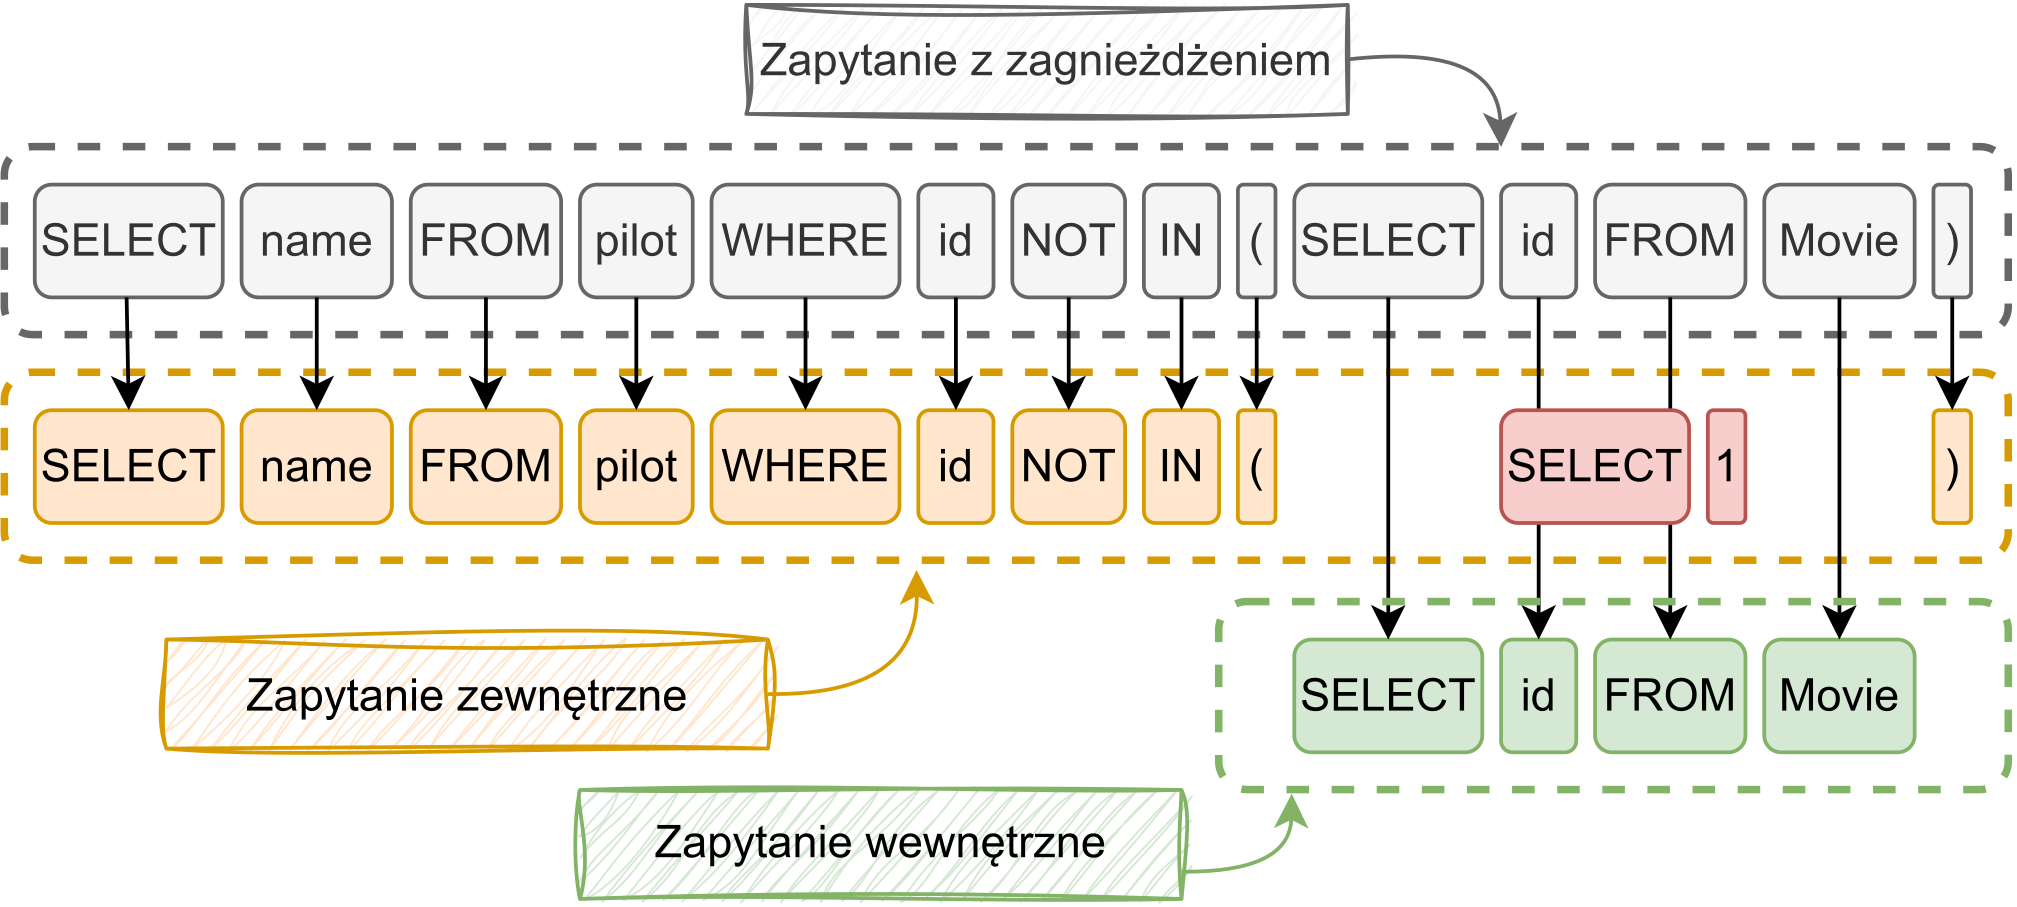
\includegraphics[width=1.0\linewidth]{images/query_decomposition_nested.png}
  \caption{Metoda dekomponowania zapytań zagnieżdżonych}
  \label{fig:query-decomposition-nested}
\end{figure}

\subsection{Dodawanie informacji redundantnych}
Jak zostało wcześniej wspomniane i zademonstrowane na listingach z źródłowych danych wykorzystywanych do generowania finalnego zbioru zostały usunięte informacje redundantne, aby umożliwić łatwiejsze wprowadzanie modyfikacji. W procesie ostatecznej syntezy należy jednak te informacje ponownie odtworzyć, aby stworzony zbiór w żaden sposób nie odbiegał formatem od oryginalnego.

Dużą część dodatkowych informacji stanowią pytania oraz zapytania SQL podzielone na tokeny. Okazuję się, że duża część istniejących rozwiązań nie wykorzystuje tych informacji, ponieważ tokenizacji można dokonać na różne sposoby i wiele rozwiązań wykonuję ją samodzielnie, wybierając sposób dla siebie najkorzystniejszy. Nie mniej jednak pierwsze modele, jak i zapewne część nowszych, korzysta z dostarczonego w ramach zbioru sposobu tokenizacji, więc należy o ten aspekt zadbać.

\subsubsection{Tokenizacja pytań}
Pytania podzielone na tokeny występują w próbkach pod kluczem \code{question\_toks}. Tokenizacji postanowiono dokonać za pomocą dostarczonego w ramach biblioteki \code{spaCy} wielojęzycznego modelu. Wybrano akurat model wielojęzyczny, a nie polski, ponieważ założono, że tworzony skrypt ma mieć możliwość generowania w razie potrzeby zbiorów z pytaniami angielskimi. Porównano jednocześnie rezultaty tokenizacji polskich pytań za pomocą modelu wielojęzycznego oraz polskiego. Okazuję się, że wyniki różnią się jedynie w niewielkiej liczbie przypadków, co świadczy o tym, że model wielojęzyczny jest dość wysokiej jakości.

\subsubsection{Tokenizacja zapytań SQL}
Kolejnym elementem, który trzeba dodać do wynikowego zbioru są zapytania SQL podzielone na tokeny. Występują one wewnątrz próbek pod kluczem \code{question\_toks}. Zaimplementowany sposób tokenizacji głównie opiera się na podzieleniu zapytań SQL na poszczególne elementy składowe, takie jak słowa kluczowe \sql{SELECT}, \sql{FROM}, \sql{WHERE}, czy nazwy tabel i kolumn. Wyjątkiem są występujące wewnątrz zapytań wartości tekstowe, które dzielone są na tokeny przy pomocy wielojęzycznego modelu z biblioteki \code{spaCy}, wspomnianego przy okazji omawiania tokenizacji pytań. Opisany proces został zilustrowany na rysunku \ref{fig:query-tokenization}.

\begin{figure}[ht!]
  \centering
  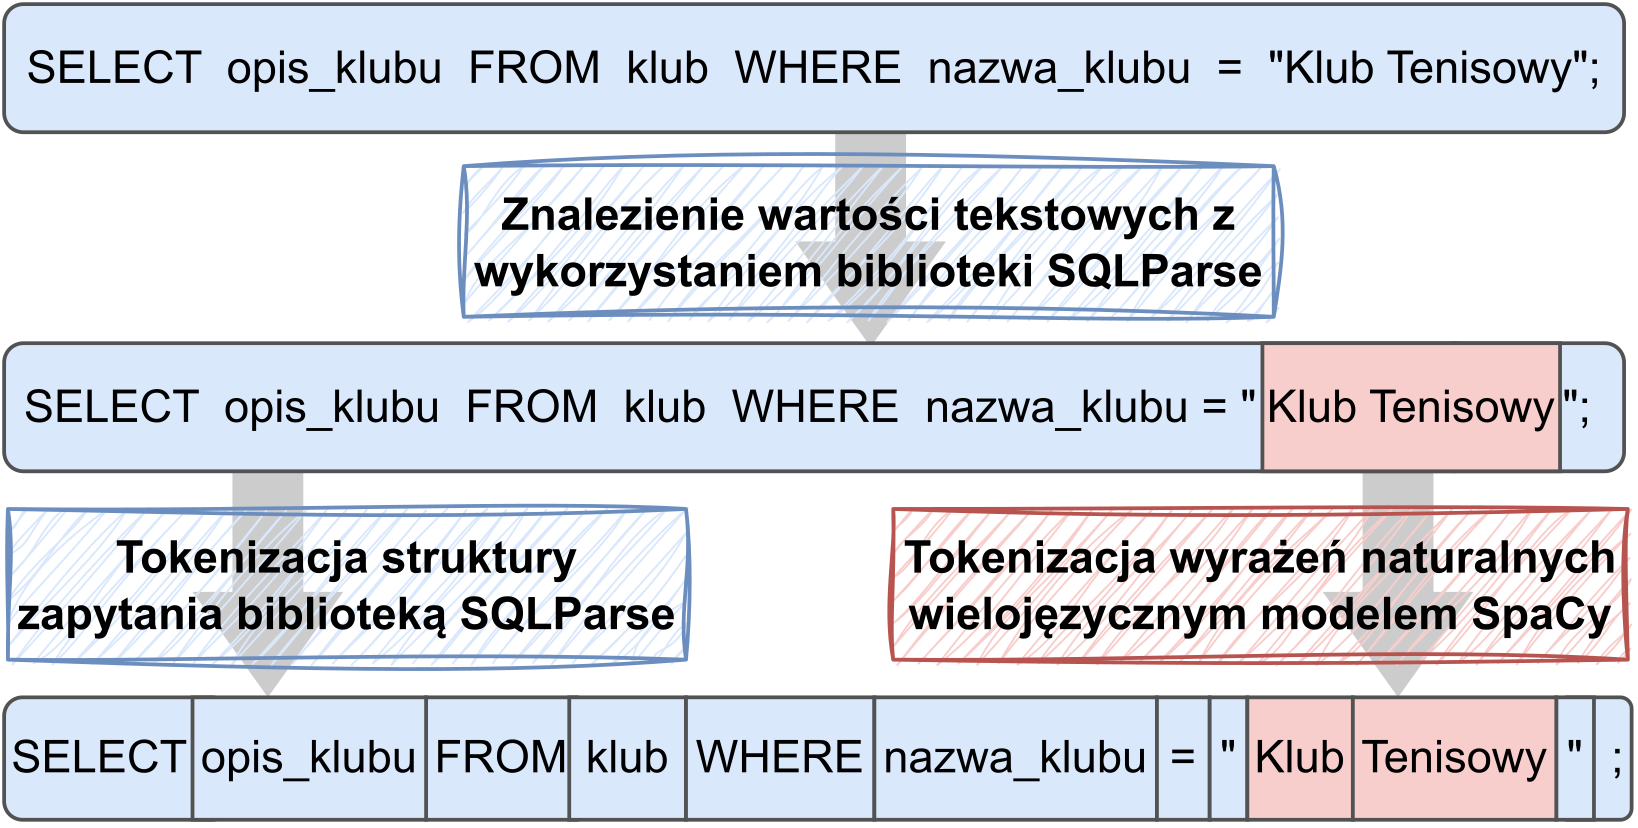
\includegraphics[width=1.0\linewidth]{images/query_tokenization.png}
  \caption{Schemat zaimplementowanej strategii tokenizacji zapytań SQL}
  \label{fig:query-tokenization}
\end{figure}

\subsubsection{Tokenizacja zapytań SQL bez wartości}
Próbki w zbiorze \code{Spider} posiadają także atrybut o nazwie \code{query\_toks\_no\_value}, który powinien zawierać zapytanie SQL podzielone na tokeny, ale bez wartości, a dokładnie wartości powinny zostać zamaskowane za pomocą specjalnego tokena \code{value}. Została więc wykorzystana ta sama technika co do standardowej tokenizacji zapytań, lecz dodatkowo wszystkie wartości zostały znalezione z wykorzystaniem biblioteki \code{sqlparse} i zamaskowane.

Opracowany algorytm jest niemal całkowicie zbieżny z wykorzystanym w oryginalnym zbiorze \code{Spider} sposobem tokenizacji. Aby to zweryfikować za jego pomocą dokonano tokenizacji oryginalnych zapytań i sprawdzono, czy wyniki pokrywają się z oryginalnymi tokenami. Okazuję się, że różnice występują jedynie w 18 przypadkach spośród prawie dziesięciu tysięcy. Sposób tokenizacji tych kilkunastu oryginalnych zapytań wyraźnie odbiega od całej reszty i przypuszcza się, że jest to niespójność oryginalnego zbioru. 

\subsubsection{Parsowanie zapytań SQL}
Ostatnim elementem, który należy dodać do zbioru są sparsowane zapytania SQL, występujące w próbkach pod kluczbem \code{sql}. Tym razem istnieje publicznie dostępny skrypt, który dokonuje tego procesu. Zostały napotkane jednak pewne problemy wynikające z jego niedociągnięć. W jednym z pierwszych kroków dokonuje on wydobycia z zapytania aliasowania, czyli słownika mówiącego jakie występują w nim aliasy i na jakie tabele się mapują. Niestety dokonuje tego globalnie, a jak zostało przedyskutowane wcześniej, nie sprawdzi się to dla wszystkich zapytań, ponieważ występują w nich zakresy - w jednej części zapytania dany alias może mapować się na zupełnie inną tabelę niż w drugiej części. Podczas uruchamiana tego skrypt na zapytaniach ze zbioru \code{Spider} (co jest najczęstszym scenariuszem jego wykorzystania) nie zwraca on żadnych błędów. Przypuszcza się, że kłopotliwe zapytania zostały ręcznie poprawione, by stały się parsowalne. W przypadku jednak, gdy zapytania zostaną wcześniej poddane tłumaczeniu nazw schematu, to problem ten wychodzi na wierzch i parsowanie kończy się najczęśniej dla kilku zapytań niepowodzeniem. 

Nasuwające się rozwiązania powyższego problemu są dwa: można poprawić skrypt parsujący lub zmodyfikować tłumaczenia tak, aby problem się nie ujawnił. Postanowiono wybrać drugą opcję, ponieważ nie wymaga ona wiele wysiłku w odróżnieniu do skomplikowanej naprawy skryptu. Przypuszcza się, że podobny był również sposób myślenia twórców zbioru \code{Spider} - zaimplementowali uproszczony skrypt parsujący, ponieważ koszt zaimplementowania wariantu pełnego znacznie przewyższa koszt jednorazowego dostosowania kilkudziesięciu zapytań. Nie mniej jednak zauważone zachowanie zostało zgłoszone na platformie \code{GitHub} w odpowiednim repozytorium, by udokumentować i zwrócić uwagę na tą kwestię.

\section{Wykonywanie tłumaczenia}
Jeden podrozdział opisywał format źródłowych danych, a kolejny sposób generowania na ich podstawie finalnych zbiorów. Nie została jeszcze poruszona kwestia tego w jaki sposób otrzymywane są znajdujące się w tych danych źródłowych tłumaczenia, poza przyjętym założeniem co do tłumaczenia maszynowego - zostanie to przedstawione w tej części.

\subsection{Wybór tłumacza}
Ważną do podjęcia decyzją był wybór konkretnego narzędzie mającego być wykorzystanym do tłumaczenia maszynowego. Obecnie większość tego typu rozwiązań bazuje na uczeniu głębokim. Są one zazwyczaj zastrzeżone i dostęp do nich uzyskuje się za pomocą webowego API. Istnieją również narzędzia typu \code{open source}, które można uruchomić w całości na własnym urządzeniu. Pozwalają uniknąć naliczania kosztów i dają możliwość swojej modyfikacji. Oferują za to mniejszą dokładność i dlatego postanowiono zrezygnować z tej drogi.

Podczas podejmowania ostatecznej decyzji wybór ograniczono do popularnych i renomowanych rozwiązań, takich jak \code{Google Cloud Translation API} \cite{google-translation-api}, \code{Microsoft Azure AI Translator} \cite{microsoft-translator}, \code{Amazon Translate API} \cite{amazon-translator} oraz \code{DeepL} \cite{deepl}. W szczególności to ostatnie wydaje się aktualnie wychodzić na prowadzenie pod względem jakości produkowanych tłumaczeń. Według informacji zawartych na swojej stronie \code{DeepL} generuje tłumaczenia ponad 3 razy dokładniejsze od rozwiązań konkurencji. Wysoką ich jakość potwierdzają również liczne artykuły naukowe \cite{Yulianto2021}\cite{Ternero2021}\cite{Bahasa2023}, które powstały na fali zachwytu tym rozwiązaniem. Posiada nawet dedykowaną bibliotekę do języka \code{Python}, ułatwiającą jego wykorzystanie. 

Jedynym aspektem, który może zniechęcać do wykorzystania \code{DeepL} są związane z tym koszty. W czasie tworzenia niniejszej pracy podstawowy plan opierał się na bazowej opłacie w kwocie 20 złotych na miesiąc oraz dodatkowym obciążeniu wynoszącym prawie 90 złotych za każdy przetłumaczony milion znaków. Dostępny jest jednak również darmowy plan, pozwalający na przetłumaczenie pół miliona znaków każdego miesiąca za darmo.

To właśnie \code{DeepL} zostało ostatecznie wybranym narzędziem, a głównym tego powodem jest niekwestionowana jakość produkowanych przez nie tłumaczeń. Oszacowano, że dostępne w ramach darmowego planu limity powinny pozwolić na zrealizowanie postawionych celów. Nie uda się to jednak w jeden miesiąc, a konieczne będzie rozłożenie tłumaczeń na dłuższy okres.

\subsection{Tłumaczenie nazw schematu}
Okazuje się, że tłumaczenie nazw tabel i kolumn jest trudnym zadaniem i z tego powodu zostało ono podzielone na dwa etapy. Pierwszy zakłada wykorzystanie tłumacza maszynowego, a drugi ręczne poprawienie tłumaczeń. W tym przypadku to ostatnie nie polega jednak na przeglądaniu każdego tłumaczenia jedno po drugim, lecz na bardziej heurystycznym podejściu, które zostanie dokładniej opisane.

\subsubsection{Tłumaczenie maszynowe}
Jako zostało wcześniej zaznaczone, w zbiorze \code{Spider} dla tabel i kolumn występują podwójne nazwy: oryginalnie występujące w bazie danych (\code{first\_name}) oraz w czytelnej, naturalnej postaci (\code{first name}). O ile przetłumaczenie tych ostatnich nie stanowi większego problemu, to nazwy oryginalne wymagają podjęcia dodatkowych akcji, ponieważ \code{DeepL} nie poradzi sobie z nimi w tej postaci - jako tłumaczenie zwróci te same nazwy, bez dokonywania żadnych zmian (\code{first\_name}), ponieważ potraktuje je jako nazwy własne, które nie podlegają tłumaczeniu. Zauważono, że \code{Google Cloud Translation} wykazuję pod tym kątem bardziej pożądane zachowanie, ale wciąż nie można by było na nim polegać. 

Aby poradzić sobie z zarysowanym problemem postanowiono przed tłumaczeniem dokonywać w nazwach podmiany znaków podkreślenia na spacje, by przekonwertować je do postaci naturalnej, a po tłumaczeniu spacje z powrotem zamieniać na znaki podkreślenia, co przedstawione zostało na rysunku \ref{fig:multi-word-translation}. Mechanizm ten nie sprawdził się dla wszystkich przypadków, ponieważ niektóre wielowyrazowe nazwy były zapisywane za pomocą innych konwencji niż oddzielanie słów znakiem podkreślenia. Były one jednak w mniejszości i tymi niedociągnięciami postanowiono się zająć na etapie ręcznych poprawek.

\begin{figure}[ht!]
  \centering
  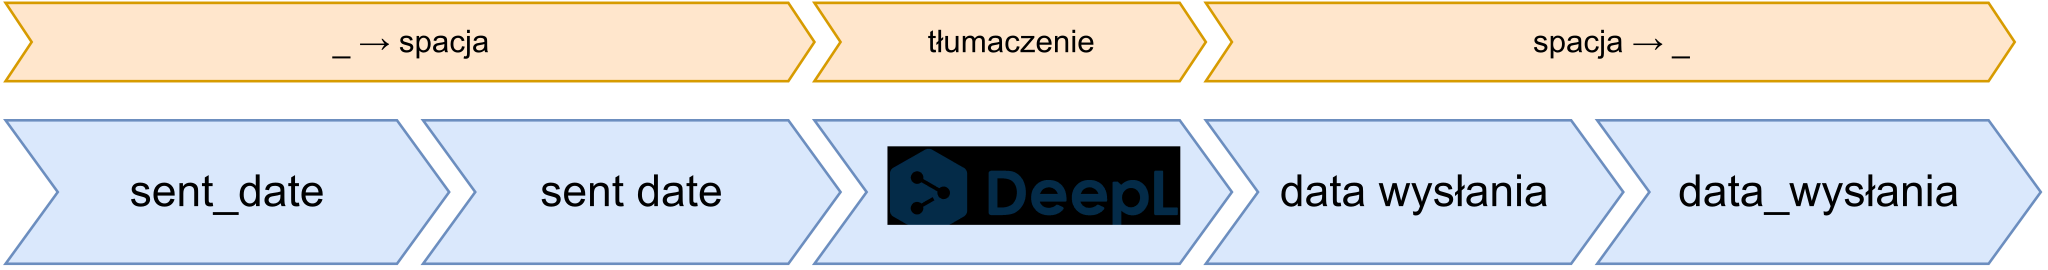
\includegraphics[width=1.0\linewidth]{images/multi_word_translation.png}
  \caption{Schemat algorytmu do tłumaczenia oryginalnych nazw tabel i kolumn}
  \label{fig:multi-word-translation}
\end{figure}

Podstawowa metoda tłumaczenia nazw to ich proste i intuicyjne przekazywanie do tłumacza. Jest to sposób, który został prawdopodobnie wykorzystany we wszystkich tłumaczeniach maszynowych zbioru \code{Spider}, ponieważ ich autorzy nie zwrócili szczególnej uwagi na tą kwestię. Podczas realizacji niniejszej pracy zauważono jednak, że wiele błędów w takich tłumaczeniach wynika z braku uwzględniania przez tłumacza kontekstu i opracowano metodę, która pozwala w dużej mierze obejść ten problem. Dla przykładu kolumna \code{home\_games}, podstawową metodą jest tłumaczona jako \code{gry\_domowe}, natomiast ulepszona metoda kontekstowa weźmie pod uwagę, że kolumna znajduję się w tabeli \code{stadium} oraz bazie danych \code{game\_injury} i tym razem nazwa zostanie przetłumaczona jako \code{mecze\_u\_siebie}.

Metoda kontekstowa polega na obserwacji, że nowoczesne narzędzia bazujące na sieciach neuronowych, w szczególności \code{DeepL}, tłumaczą to samo słowo w różny sposób w zależności od kontekstu w jakim ono wystąpiło. Z tego powodu do tłumacza poza samymi nazwami tabel i kolumn postanowiono także podawać w roli kontekstu nazwy baz danych, a dla kolumn również nazwy tabeli. Zostały opracowane szablony, które służą do tworzenia skontekstualizowanych wyrażeń podawanych do tłumacza i wraz z przykładami użycia zostały przedstawione na rysunku \ref{fig:translation-in-context}. Dla porównania postanowiono dokonać tłumaczenia bezkontekstowego i okazało się, że wynikowe tłumaczenia nazw pomiędzy tymi metodami różnią się dla 21,41\% przypadków, co stanowi dużą różnicę.

\begin{figure}[ht!]
\centering
\begin{subfigure}{0.4\textwidth}
    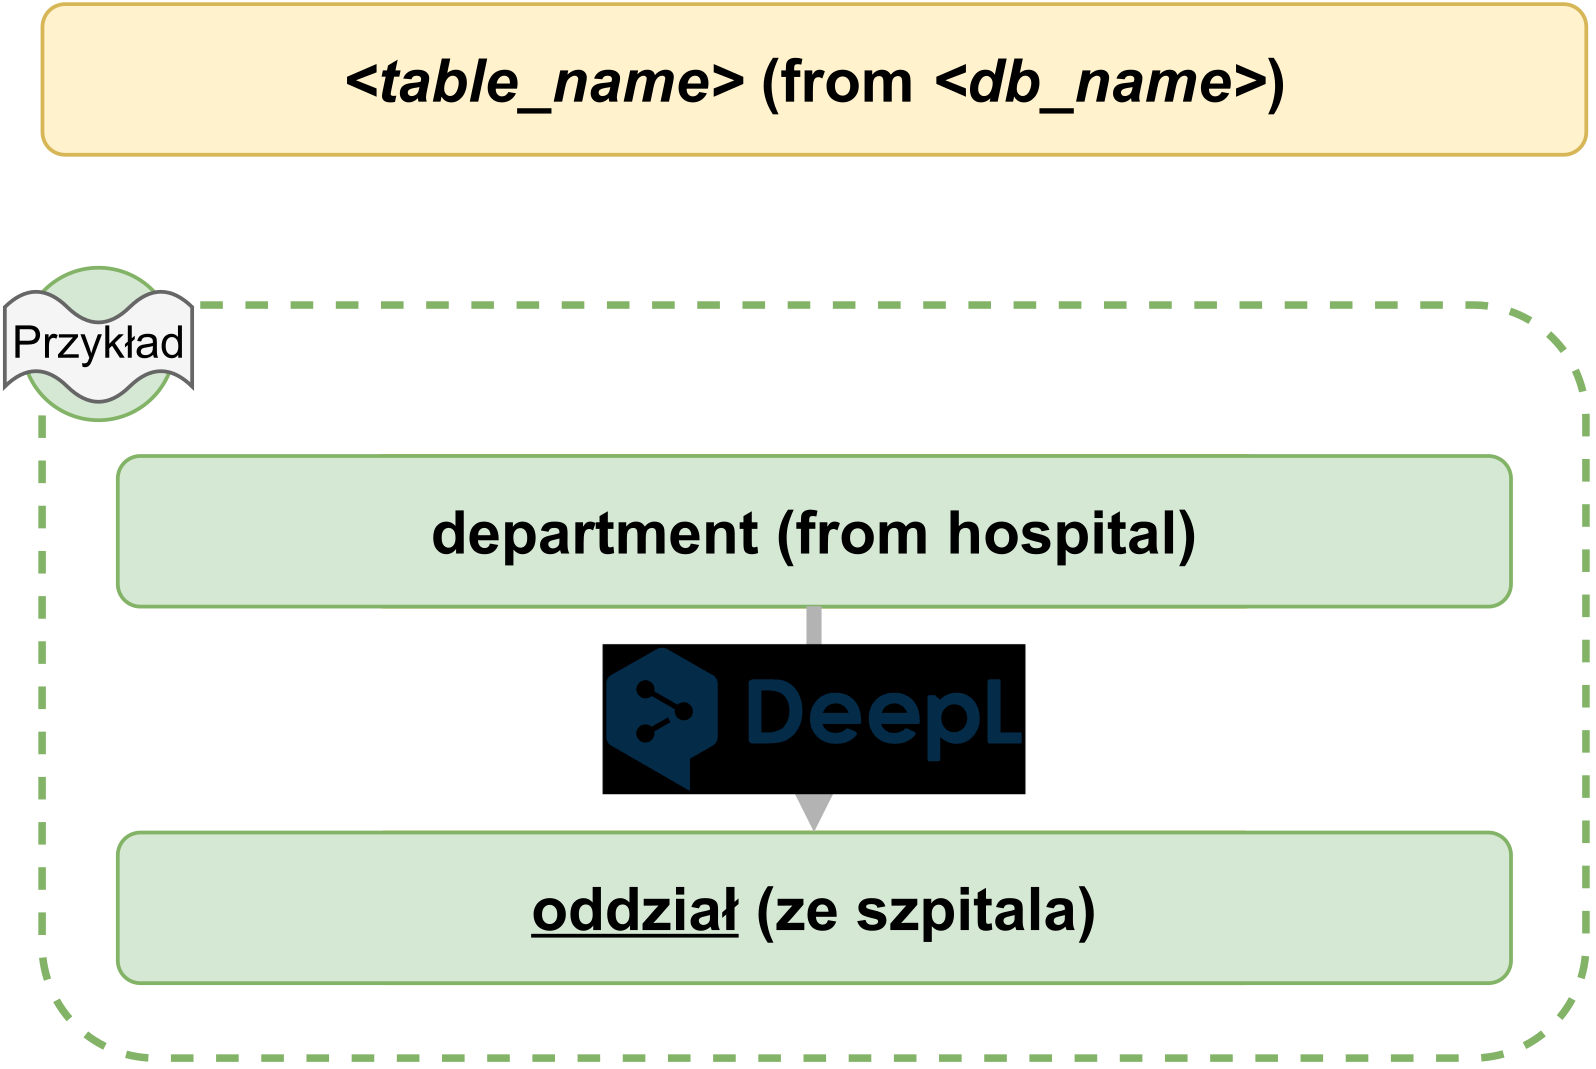
\includegraphics[width=\textwidth]{images/translation_in_context_table.png}
    \caption{Dla tabel}
    \label{fig:first}
\end{subfigure}
\hfill
\begin{subfigure}{0.50\textwidth}
    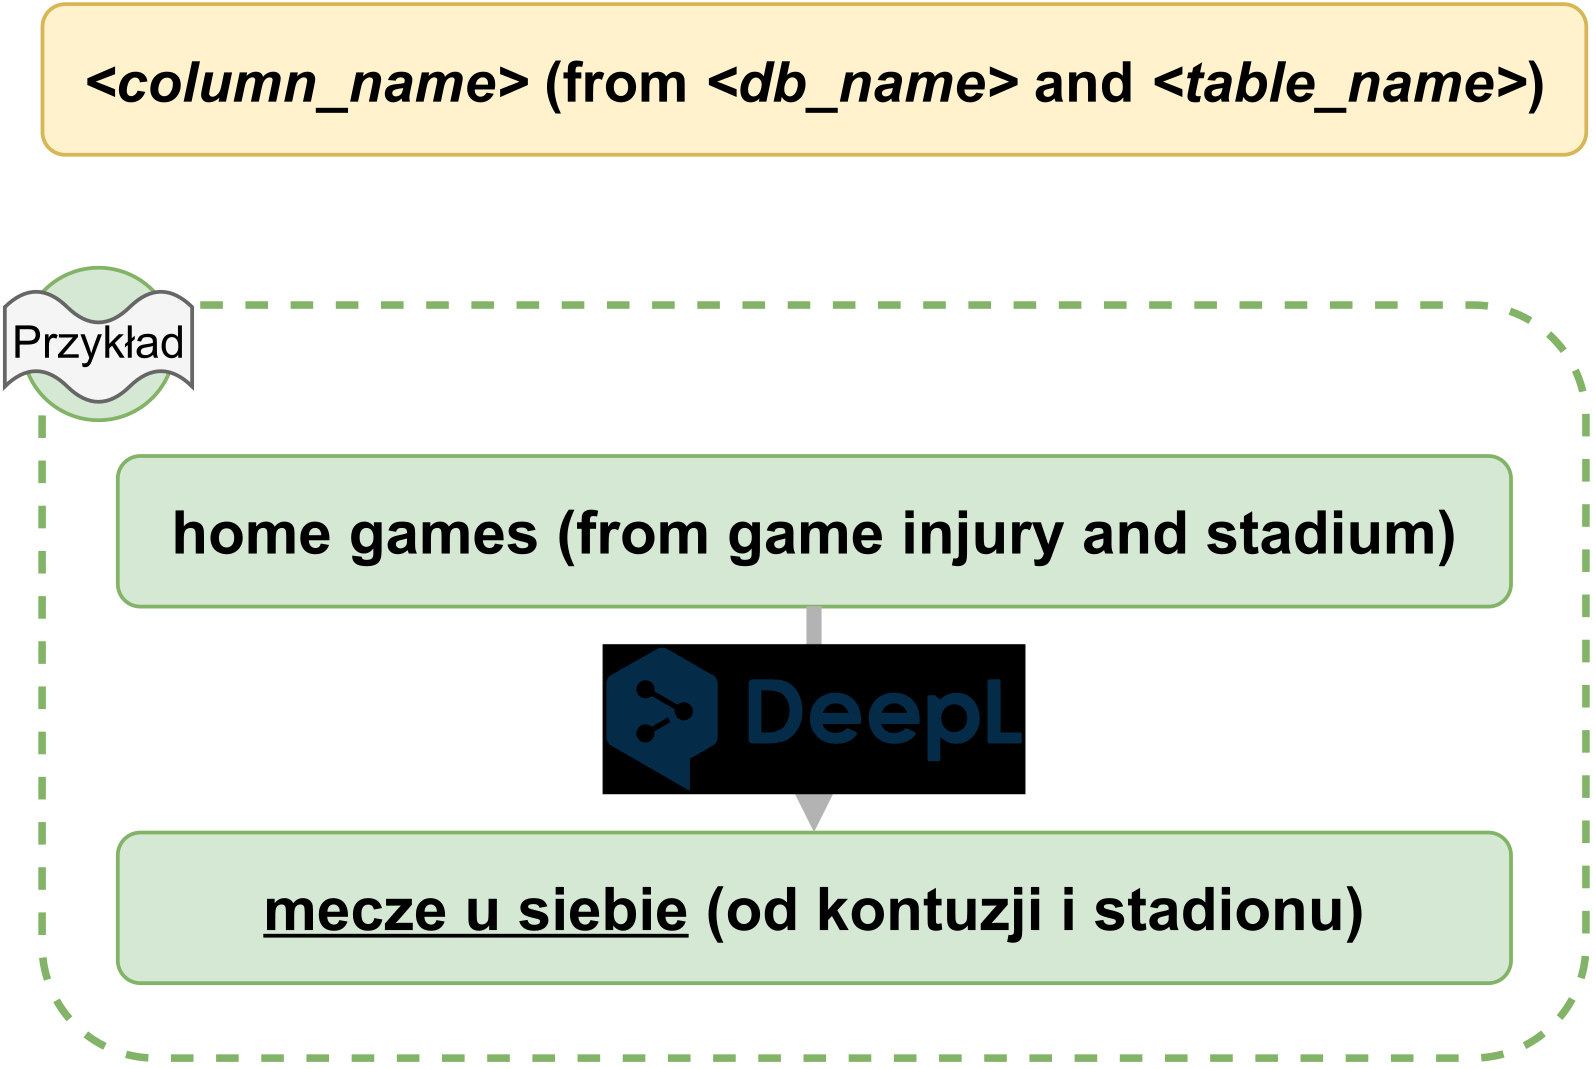
\includegraphics[width=\textwidth]{images/translation_in_context_column.png}
    \caption{Dla kolumn}
    \label{fig:second}
\end{subfigure}
\caption{Szablony do tłumaczenia kontekstowego}
\label{fig:translation-in-context}
\end{figure}

Przedstawiona strategia tłumaczenia kontekstowego jest zainspirowana metodą \code{SAVe}, opisaną w artykule dotyczącym wielojęzycznego zbioru \code{MultiSpider} \cite{Dou2022}. Została tam wykorzystana jako metoda augmentacji w celu poprawienia osiąganych przez model wyników. Jest bardziej skomplikowana od przedstawionego powyżej wariantu, ponieważ zakłada wykorzystanie wielu szablonów oraz ma dodatkowych etap weryfikacji tłumaczeń, co jednak dla rozważanego problemu nie ma dobrego uzasadnienia.

Oczywistym minusem zaproponowanej metody jest istotne zwiększenie długości tekstów podawanych do tłumacza, co w przypadku \code{DeepL} wpływa na naliczenie wyższych kosztów lub też szybsze wykorzystanie darmowych limitów - na co się mimo wszystko zdecydowano. Zaletą strategii kontekstowej jest poprawa tłumaczenia dla wielu nazw, jednak z pewnego punktu widzenia może ona także wpływać na obniżenie czytelności przetłumaczonego schematu. Zdarzają się bowiem przypadki, iż w obrębie jednej bazy pewna nazwa kolumny zostaje przetłumaczona na kilka różnych sposobów, chociaż nie powinna. Zmniejsza to spójność tak przetłumaczonego schematu, bo sugeruje, że przechowywane są w tych kolumnach dane o różnym znaczeniu, a w rzeczywistości jest inaczej. Nie jest więc banalnym oszacowanie wypadkowego wpływu zastosowania tej metody na jakość finalnego zbioru, uważa się jednak, że jest on pozytywny.

\subsubsection{Ręczne poprawki}
Po uzyskaniu tłumaczeń maszynowych nazw tabel i kolumn oraz ich wstępnej ocenie było oczywistym, że wciąż zawierają pewne błędy. Przejrzenie każdego z nich jedno po drugim wymagałoby znacznego nakładu czasu, więc postanowiono posłużyć się metodami heurystycznymi, by zlokalizować tylko te najbardziej podejrzane. 

Zauważono, że dla błędnych tłumaczeń bardzo często nazwa przetłumaczona jest identyczna z angielską, więc korzystając z tego faktu, prostych skryptów oraz możliwości edytora \code{Visual Studio Code} dokonano znalezienia właśnie takich przypadków, a następnie je poprawiono. Były to w dużej mierze nazwy składające się z kilku wyrazów połączonych ze sobą za pomocą innej konwencji niż znaki podkreślenia, bo tylko ten najpopularniejszy wariant był obsługiwany w fazie maszynowej. Dość częste były również kilkuliterowe skróty jak \code{mid} (movie id), czy \code{aid} (author id), z którymi - co nie dziwi - \code{DeepL} sobie nie poradził. Poza tym dokonano poprawy kilkunastu wyrażeń w przypadku których zaobserwowano częste pomyłki, jak tłumaczenie \code{name} na \code{imię i nazwisko}, chociaż powinno zostać przetłumaczone jako \code{nazwa}, czy \code{id}, które niepotrzebnie zostało przetłumaczone na rozwlekłą nazwę \code{identyfikator}.

Na cały etap ręcznych poprawek zostało poświęcone kilka godzin i w jego wyniku zmodyfikowanych zostało 10,54\% tłumaczeń maszynowych. Wydaje się to dużą częścią, lecz większość z tych modyfikacji dokonano w szybki, półautomatyczny sposób.


\subsection{Tłumaczenie pytań}
Tłumaczenie pytań sprowadza się do uzupełnienia w przedstawionym wcześniej formacie próbek wartości \code{question.pl} na podstawie atrybutu \code{question.en}. W tym przypadku pytania zostały bezpośrednio przekazane do tłumacza, bez stosowania żadnych dodatkowych sztuczek. Uznano, że stosowanie tłumaczenia kontekstowego, które oznaczałoby rozszerzenie przekazywanych do tłumacza tekstów o nazwę bazy danych z której pochodzą, nie ma sensu. Wiązałoby się to z tłumaczeniem większej liczby znaków na podstawie których \code{DeepL} obciąża swoich użytkowników, a uzyskana poprawa prawdopodobnie nie byłaby znacząca. Pytania są bowiem zwykle na tyle długie, że pozwalają tłumaczowi na wywnioskowanie domeny której dotyczą i wybranie odpowiednich tłumaczeń dla problematycznych słów. 

Etap manualnych poprawek nie został w tym przypadku wykorzystany, gdyż pytania zawierają dużą ilość tekstu i ciężko jest dostrzec w nich ewentualne błędy. Nie znaleziono również żadnych sposobów na znalezienie podejrzanych tłumaczeń, czy dokonanie półautomatycznych poprawek, tak jak to miało miejsce dla tłumaczenia nazw tabel i kolumn. Ostatecznie maszynowe tłumaczenia pytań wydawały się na tyle wysokiej jakości, że postanowiono przejść do kolejnych etapów.

\subsection{Tłumaczenie wartości w zapytaniach SQL}
Tłumaczenie wartości w zapytaniach SQL odbyło się poprzez uzupełnienie atrybutów \code{query.pl} na podstawie \code{query.en} w pliku z próbkami o przedstawionym wcześniej formacie. Ten ostatni atrybut zawiera oryginalne zapytania SQL, natomiast pierwszy zapytania z wszelkimi anglojęzycznymi łańcuchami znaków przetłumaczonymi na język polski.

W celu znalezienia w danym zapytaniu wartości tekstowych dokonywano jego przetwarzania z wykorzystaniem biblioteki \code{sqlparse}. Pozwalała ona podzielić zapytanie na poszczególne tokeny i wybrać te, które posiadają typ \code{Token.Literal.String}, czyli właśnie wartości tekstowe. Są to wyrażenia zamknięte w pojedynczych lub podwójnych cudzysłowach, które przekazywano do \code{DeepL} w celu uzyskania tłumaczeń, a następnie zastępowano nimi oryginalne teksty. Wyjątek stanowią jedynie wartości występujące w roli szablonów po słowie kluczowym \code{LIKE}, takie jak \code{'\%Hey\%'}, \code{'\%East\%'}, \code{'S\%'}. Nie są one zapisane w języku naturalnym, ponieważ zawierają specjalne znaki, stanowiące problem dla tłumacza maszynowego. Z tego względu, a także biorąc pod uwagę rzadkość takich przypadków, postanowiono przetłumaczyć je manualnie. Wizualizacja tego etapu została przedstawiona na rysunku \ref{fig:value-translation}

\begin{figure}[ht!]
  \centering
  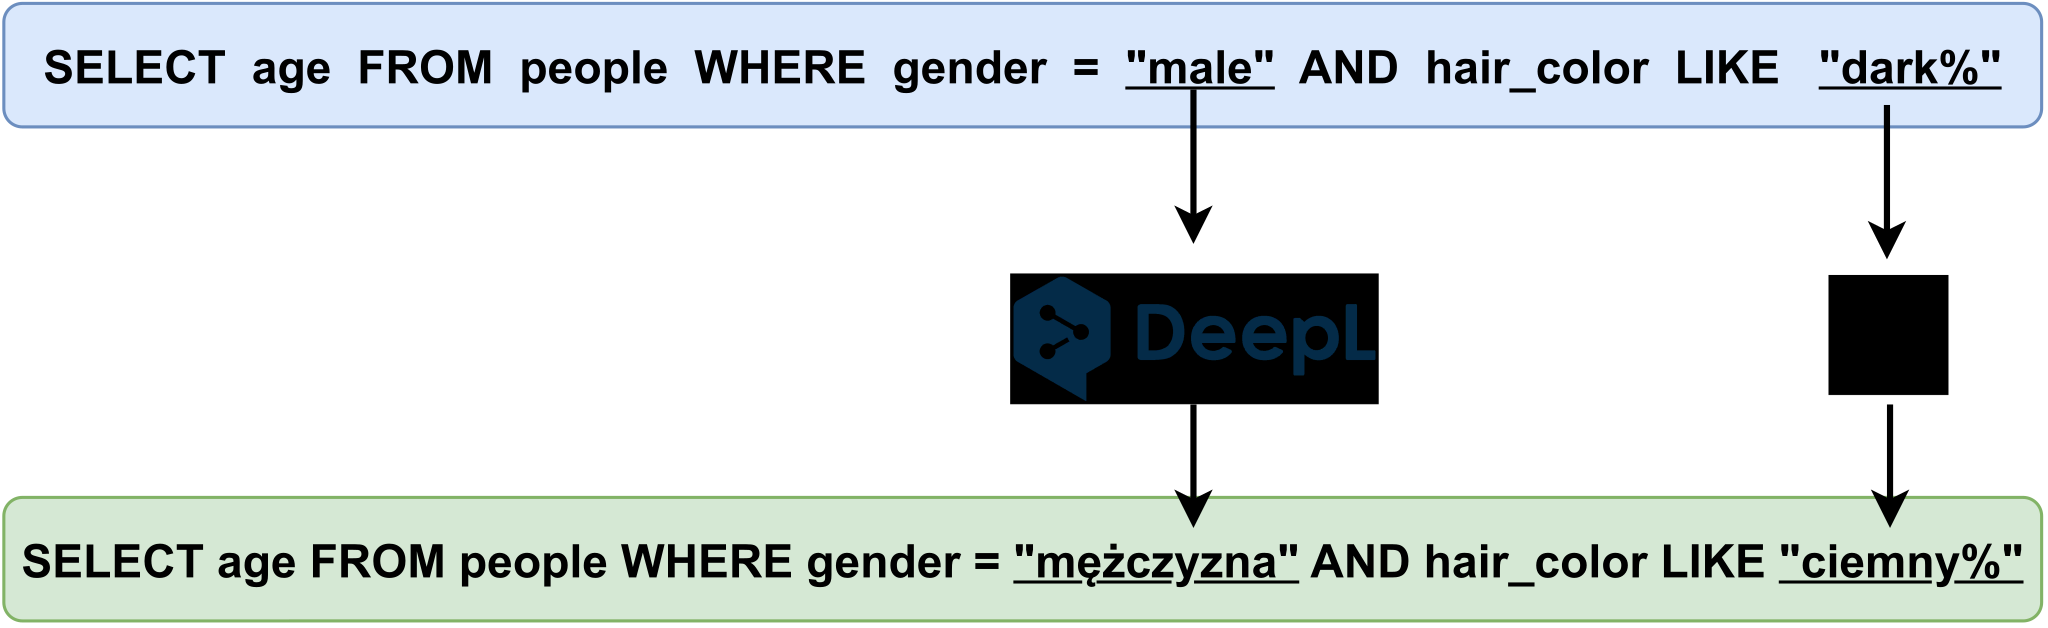
\includegraphics[width=1.0\linewidth]{images/value_translation.png}
  \caption{Wizualizacja etapu tłumaczenia wartości w zapytaniach SQL}
  \label{fig:value-translation}
\end{figure}

\section{Podsumowanie stworzonych zbiorów}
Niniejszy podrozdział stanowi ukoronowanie pracy nad polskimi zbiorami danych, ponieważ zawiera on przedstawienie i analizę przygotowanych zbiorów przykładów, tłumaczeń schematów oraz ostatecznie zbiorów, które poprzez ich kombinację można wygenerować.

\subsection{Przygotowane zbiory przykładów}

% \begin{table}[ht]
%     \centering
%     \begin{tabular}{|l|c|c|c|c|}
%         \hline
%         \thead{Zbiór} & 
%         \thead{Rodzaj\\tłumaczenia} &
%         \thead{Tłumaczenie\\schematu} &
%         \thead{Tłumaczenie\\zawartości\\baz danych} &
%         \thead{Tłumaczenie\\wartości w\\zapytaniach} \\
%         \hline
%         \makecell{Chiński\\(\code{CSpider})} & Manualne & Nie & Nie & Tak \\
%         \hline
%         \makecell{Wietnamski\\(\code{ViText2SQL})} & Manualne & Tak & Nie & Tak \\
%         \hline
%         \makecell{Portugalski} & Maszynowe & Tak & Nie & Nie \\
%         \hline
%         \makecell{Rosyjski\\(\code{PAUQ})} & Manualne & Nie & Częściowo & Tak \\
%         \hline
%     \end{tabular}
%     \caption{Zestawienie kluczowych różnic pomiędzy tłumaczeniami zbioru \code{Spider}}
%     \label{tab:spider-trans-diffs}
% \end{table}

\begin{table}[ht]
    \centering
    \begin{tabular}{|l|R{0.15\textwidth}|R{0.15\textwidth}|R{0.15\textwidth}|}
        \hline
        \thead{Zbiór} & \thead{Część\\treningowa} & \thead{Część\\walidacyjna} & \thead{Razem} \\
        \hline
        Spider & 8659 & 1034 & 9693 \\
        \hline
        Spider-DK & 0 & 535 & 535 \\
        \hline
        Spider-Syn & 3556 & 773 & 4329 \\
        \hline
        CoSQL & 1562 & 230 & 1792 \\
        \hline
        SParC & 2651 & 366 & 3017 \\
        \hhline{|=|=|=|=|} 
        Razem & 16428 & 2938 & 19366 \\
        \hline
    \end{tabular}
    \caption{Zestawienie liczby próbek w poszczególnych zbiorach}
    \label{tab:samples-count}
\end{table}

\begin{table}[ht]
    \centering
    \begin{tabular}{|l|R{0.15\textwidth}|R{0.15\textwidth}|R{0.15\textwidth}|R{0.15\textwidth}|R{0.15\textwidth}|}
        \hline
        \thead{Zbiór} & \thead{Easy} & \thead{Medium} & \thead{Hard} & \thead{Extra hard} \\
        \hline
        Spider & 2231 (23\%) & 3445 (36\%) & 2095 (22\%) & 1922 (20\%) \\
        \hline
        Spider-DK & 110 (21\%) & 246 (46\%) & 74 (14\%) & 105 (20\%) \\
        \hline
        Spider-Syn & 952 (22\%) & 1825 (42\%) & 884 (20\%) & 668 (15\%) \\
        \hline
        CoSQL & 949 (53\%) & 488 (27\%) & 222 (12\%) & 133 (\s7\%) \\
        \hline
        SParC & 2131 (71\%) & 706 (23\%) & 138 (\s5\%) & 42 (\s1\%) \\
        \hhline{|=|=|=|=|=|} 
        Wszystkie & 6373 (33\%) & 6710 (35\%) & 3413 (18\%) & 2870 (15\%) \\
        \hline
    \end{tabular}
    \caption{Zestawienia liczby próbek o poszczególnych poziomach trudności}
    \label{tab:difficulty}
\end{table}

% \begin{table}[ht]
%     \centering
%     \begin{tabular}{|l|R{0.15\textwidth}|R{0.15\textwidth}|R{0.15\textwidth}|}
%         \hline
%         \thead{Zbiór} & \thead{Min} & \thead{Max} & \thead{Średnia} \\
%         \hline
%         Spider & 3\s / \s3 & 224 / 227 & 66,74 / 66,44 \\
%         \hline
%         Spider-DK & 21 / 15 & 152 / 159 & 66,01 / 65,93 \\
%         \hline
%         Spider-Syn & 20 / 16 & 222 / 234 & 74,03 / 74,14 \\
%         \hline
%         CoSQL & 17 / 14 & 147 / 201 & 53,05 / 52,66 \\
%         \hline
%         SParC & 15 / 13 & 122 / 139 & 44,94 / 45,52 \\
%         \hhline{|=|=|=|=|} 
%         Wszystkie & 3\s / \s3 & 224 / 234 & 63,69 / 63,61 \\
%         \hline
%     \end{tabular}
%     \caption[Zestawienie liczby znaków polskich i angielskich pytań]{Zestawienie liczby znaków polskich i angielskich pytań (en / pl)}
%     \label{tab:questions-lengths}
% \end{table}

% \begin{table}[ht]
%     \centering
%     \begin{tabular}{|l|R{0.15\textwidth}|R{0.15\textwidth}|R{0.15\textwidth}|}
%         \hline
%         \thead{Zbiór} & \thead{Min} & \thead{Max} & \thead{Średnia} \\
%         \hline
%         Spider & 2 / 2 & 58 / 63 & 10,66 / 11,28 \\
%         \hline
%         Spider-DK & 3 / 3 & 28 / 28 & 8,47 / 8,59 \\
%         \hline
%         Spider-Syn & 2 / 2 & 39 / 54 & 9,65 / 10,28 \\
%         \hline
%         CoSQL & 3 / 3 & 51 / 66 & 10,11 / 10,72 \\
%         \hline
%         SParC & 3 / 3 & 45 / 55 & 10,24 / 10,84 \\
%         \hhline{|=|=|=|=|} 
%         Wszystkie & 2 / 2 & 58 / 66 & 10,32 / 10,94 \\
%         \hline
%     \end{tabular}
%     \caption[Zestawienie liczby znaków polskich i angielskich wartości z zapytań]{Zestawienie liczby znaków polskich i angielskich wartości z zapytań (en / pl)}
%     \label{tab:questions-lengths}
% \end{table}

\begin{table}[ht]
    \centering
    \begin{tabular}{|l|R{0.15\textwidth}|R{0.15\textwidth}|R{0.15\textwidth}|}
        \hline
        \thead{Zbiór} & \thead{Pytania} & \thead{Wartości} \\
        \hline
        Spider & 66,74 / 66,44 & 10,66 / 11,28 \\
        \hline
        Spider-DK & 66,01 / 65,93 & \s8,47 / \s8,59 \\
        \hline
        Spider-Syn & 74,03 / 74,14 & 9,65 / 10,28 \\
        \hline
        CoSQL & 53,05 / 52,66 & 10,11 / 10,72 \\
        \hline
        SParC & 44,94 / 45,52 & 10,24 / 10,84 \\
        \hhline{|=|=|=|} 
        Wszystkie & 63.69 / 63.61 & 10,32 / 10,94 \\
        \hline
    \end{tabular}
    \caption[Zestawienie liczby znaków w pytaniach i wartościach dla języka angielskiego i polskiego]{Zestawienie liczby znaków w pytaniach i wartościach dla języka angielskiego i polskiego (en / pl)}
    \label{tab:questions-lengths}
\end{table}

\subsection{Przygotowane tłumaczenia schematów}


\subsection{Nazwane warianty}

% Przedstawienie stworzonych zbiorów nie jest proste, ponieważ założeniem było, aby dla każdej wersji angielskiej nie powstało tylko jedno statyczne tłumaczenie, lecz aby można było wygenerować różne polskie warianty. Nie mniej jednak w celu ułatwienia dalszej pracy poprzez możliwość odwoływania się do konkretnych zbiorów to kilka wariantów zostało zdefiniowanych i nazwanych. Ponadto zdefiniowane i nazwane zostały również pewne połączenia tych zbiorów, do których występują częste odwołania. 

W celu ułatwienia dalszej pracy poprzez możliwość odwoływania się do konkretnych zbiorów kilka wariantów zbiorów zostało nazwanych. Ponadto zdefiniowane zostały również pewne połączenia tych zbiorów, ponieważ występują do nich częste odwołania.

\begin{figure}[ht!]
  \centering
  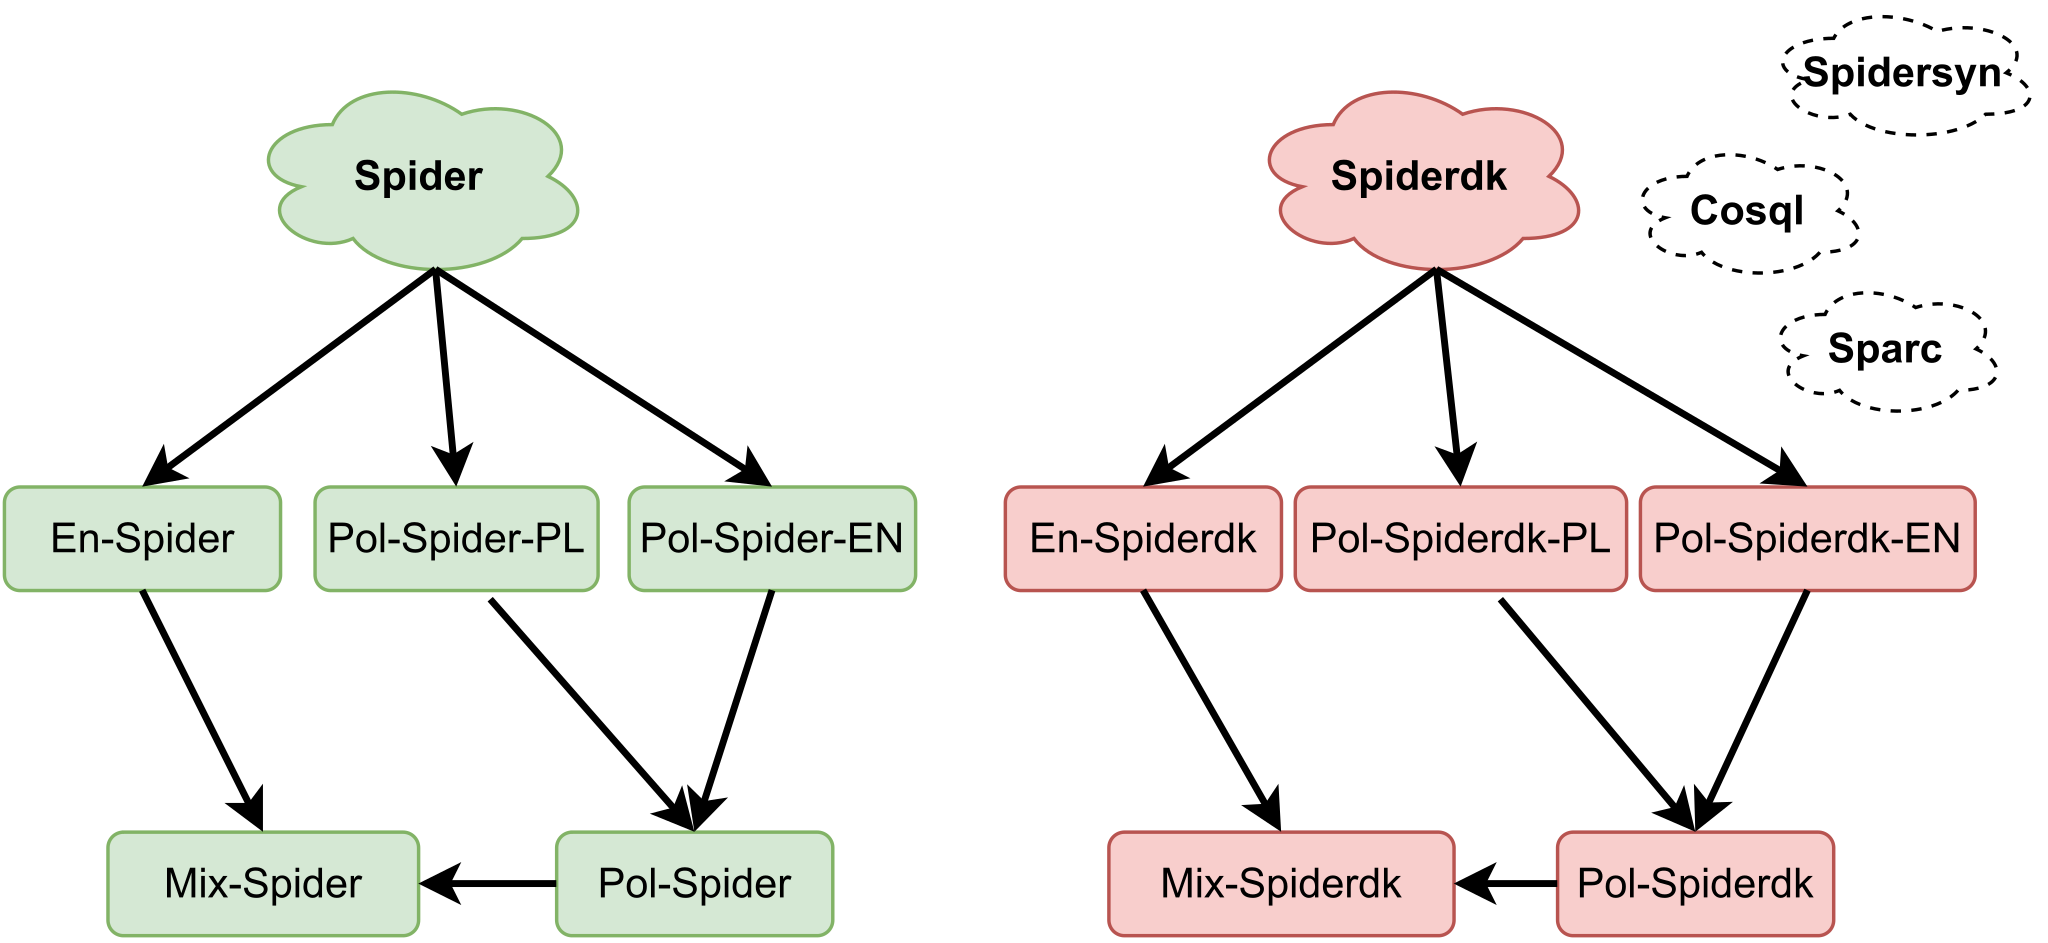
\includegraphics[width=1.0\linewidth]{images/datasets.png}
  \caption{Schemat zależności pomiędzy zbudowanymi zbiorami danych}
  \label{fig:datasets}
\end{figure}

Schemat zdefiniowanych zbiorów został przedstawiony na rysunku \ref{fig:datasets}. Można z niego odczytać, że na bazie zbioru \code{Spider} wygenerowane zostały trzy warianty. \code{En-Spider} to wariant całkowicie angielski, bardzo podobny do oryginalnego \code{Spider}, ale z minimalnymi różnicami, jak sposób tokenizacji. \code{Pol-Spider-PL} to wariant polski z polskim schematem baz danych, a \code{Pol-Spider-EN} to wariant polski z angielskim schematem baz danych. Te dwa polskie warianty zostały połączone w zbiór \code{Pol-Spider}, który jest więc polskim zbiorem zawierającym schematy baz danych w obu popularnych wariantach. Ponadto często wykorzystywane jest złączenie zbioru przetłumaczonego z angielskim więc połączenie zbioru \code{Pol-Spider} oraz \code{En-Spider} nazwano \code{Mix-Spider}. Podobny schemat nazewnictwa został zastosowany do reszty zbiorów. Schematyczne i wymowne nazwy powinny ułatwić zapamiętanie tych relacji.

% Ponadto stworzone i nazwane zostały globalne złączenia pomiędzy wszystkimi opisanymi powyżej wariantami. \code{Ultimate} zawiera wszystkie całkowicie angielskie warianty. \code{Pol-Ultimate-EN} oraz \code{Pol-Ultimate-PL} zawierają wszystkie polskie warianty z odpowiednio angielskimi i polskimi schematami baz danych. \code{Pol-Ultimate} agreguje dwa powyższe, a \code{Pol-Ultimate-Mix} dodatkowo dodaje do tego warianty angielskie. 


Należy zaznaczyć, że warianty zawierające schemat baz danych w języku polskim nie zawierają tam polskich znaków. Bezproblemowe byłoby wygenerowanie również zbiorów, które zawierałyby polskie znaki w schemacie, lecz jest to tak rzadko spotykany w praktyce przypadek, że nie był brany pod uwagę.



\fchapter{Przegląd problemu Text-to-SQL}
\fsection{Stosowane metryki}
\fsection{Wysokopoziomowe podejścia}
% \fsection{Etap schema linking}

\fchapter{Metoda RAT-SQL}
\fsection{Opis metody RAT-SQL}
\fsection{Modyfikacje dla języka polskiego}
\fsection{Eksperymenty}
\fsection{Wyniki i analiza eksperymentów}

\fchapter{Metoda Bridge}
\fsection{Opis metody BRIDGE}
\fsection{Modyfikacje dla języka polskiego}
\fsection{Eksperymenty}
\fsection{Wyniki i analiza eksperymentów}

\fchapter{Finalne rozwiązanie}
\fsection{Przebieg eksperymentu}
\fsection{Automatyczna ocena}
\fsection{Manualna ocena}

\fchapter{Podsumowanie}